% -*- latex -*-

%%%%%%%%%%%%%%%%%%%%%%%%%%%%%%%%%%%%%%%%%%%%%%%%%%%%%%%%%%%%%%%%%%%%%%%%%%%%%
% This beginning part of the preamble is specific to the
% acm document class.

%\documentclass{acm_proc_article-sp}
\documentclass{sig-alternate}

%% Paper title.

%\title{Sort-Last Smackdown!}
\title{An Image Compositing Solution At Scale}

%
% You need the command \numberofauthors to handle the 'placement
% and alignment' of the authors beneath the title.
%
% For aesthetic reasons, we recommend 'three authors at a time'
% i.e. three 'name/affiliation blocks' be placed beneath the title.
%
% NOTE: You are NOT restricted in how many 'rows' of
% "name/affiliations" may appear. We just ask that you restrict
% the number of 'columns' to three.
%
% Because of the available 'opening page real-estate'
% we ask you to refrain from putting more than six authors
% (two rows with three columns) beneath the article title.
% More than six makes the first-page appear very cluttered indeed.
%
% Use the \alignauthor commands to handle the names
% and affiliations for an 'aesthetic maximum' of six authors.
% Add names, affiliations, addresses for
% the seventh etc. author(s) as the argument for the
% \additionalauthors command.
% These 'additional authors' will be output/set for you
% without further effort on your part as the last section in
% the body of your article BEFORE References or any Appendices.

\numberofauthors{1}

% You can go ahead and credit any number of authors here,
% e.g. one 'row of three' or two rows (consisting of one row of three
% and a second row of one, two or three).
%
% The command \alignauthor (no curly braces needed) should
% precede each author name, affiliation/snail-mail address and
% e-mail address. Additionally, tag each line of
% affiliation/address with \affaddr, and tag the
% e-mail address with \email.
%% \author{
%%   %
%%   \alignauthor Kenneth Moreland \\
%%   \affaddr{Sandia National Laboratories} \\
%%   \email{kmorel@sandia.gov}
%%   %
%%   \alignauthor Wesley Kendall \\
%%   \affaddr{University of Tennessee, Knoxville} \\
%%   \email{kendall@eecs.utk.edu}
%%   %
%%   \alignauthor Tom Peterka \\
%%   \affaddr{Argonne National Laboratory} \\
%%   \email{tpeterka@mcs.anl.gov}
%%   %
%%   \and % Another row of authors.
%%   %
%%   \alignauthor Jian Huang \\
%%   \affaddr{University of Tennessee, Knoxville} \\
%%   \email{huangj@eecs.utk.edu}
%%   %
%% }

\author{
\alignauthor
Ken Moreland$^\ddagger$, Wesley Kendall$^*$, Tom Peterka$^\dagger$ and Jian Huang$^*$\\
    %\affaddr{Dept. of Electrical Engineering and Computer Science}\\
    \affaddr{$^\ddagger$Sandia National Laboratory}\\
    \affaddr{$^*$University of Tennessee, Knoxville}\\
    \affaddr{$^\dagger$Argonne National Laboratory}\\
}


% End of acm-specific portion of the preamble.
%%%%%%%%%%%%%%%%%%%%%%%%%%%%%%%%%%%%%%%%%%%%%%%%%%%%%%%%%%%%%%%%%%%%%%%%%%%%%

\usepackage{amsfonts}
\usepackage{amssymb}
\usepackage{amsmath}
\usepackage{graphicx}
\usepackage{varioref}
\usepackage{fancyvrb}
\usepackage{ifthen}
\usepackage{cite}
\usepackage{subfig}
\usepackage{xspace}
\usepackage{clrscode}
\usepackage{hyperref}
\usepackage{verbatim}

\usepackage{color}
\definecolor{yellow}{rgb}{1,1,0}
\definecolor{black}{rgb}{0,0,0}
\definecolor{ltcyan}{rgb}{.75,1,1}
\definecolor{red}{rgb}{1,0,0}

% Cite commands I use to abstract away the different ways to reference an
% entry in the bibliography (superscripts, numbers, dates, or author
% abbreviations).  \scite is a short cite that is used immediately after
% when the authors are mentioned.  \lcite is a full citation that is used
% anywhere.  Both should be used right next to the text being cited without
% any spacing.
\newcommand*{\lcite}[1]{~\cite{#1}}
\newcommand*{\scite}[1]{~\cite{#1}}

\newcommand{\etal}{et al.}

\newcommand*{\keyterm}[1]{\emph{#1}}

\newcommand{\Oh}{\mathrm{O}}

\newcommand{\sticky}[1]{{\color{red}\textsc{[#1]}}}

% Avoid putting figures on their own page.
\renewcommand{\textfraction}{0.05}
\renewcommand{\topfraction}{0.95}

% Make sure this is big enough so that only big figures end up on their own
% page but small enough so that if a figure does have to be on its own
% page, it won't push everything to the bottom because it's not big enough
% to have its own page.
\renewcommand{\floatpagefraction}{.75}

\newenvironment{packed_enum}{
\begin{enumerate}
  \setlength{\topsep}{0pt}
  \setlength{\itemsep}{0pt}
  \setlength{\parskip}{0pt}
  \setlength{\parsep}{0pt}
  \setlength{\partopsep}{0pt}
}{\end{enumerate}}

\begin{document}

\sloppy

\maketitle

\begin{abstract}
  The only proven method for performing distributed-memory parallel
  rendering at large scales, tens of thousands of nodes, is a class of
  algorithms called sort last.  The fundamental operation of sort-last
  parallel rendering is an image composite, which combines a collection of
  images generated independently on each node into a single blended image.
  Over the years numerous image compositing algorithms have been proposed
  as well as several enhancements and rendering modes to these core
  algorithms.  However, the testing of these image compositing algorithms
  has been with an arbitrary set of enhancements, if any are applied at
  all.  In this paper we take a leading production-quality
  image-compositing framework, IceT, and use it as a testing framework for
  the leading image compositing algorithms of today.  As we scale IceT to
  ever increasing job sizes, we consider the image compositing systems
  holistically, incorporate numerous optimizations, and discover several
  improvements to the process never considered before.  We conclude by
  demonstrating our system on 64K cores of the Intrepid BlueGene/P at
  Argonne National Laboratories.
\end{abstract}

%% ACM Computing Classification System (CCS). 
%% See <http://www.acm.org/class/1998/> for details.

\category{I.3.1}{Computer Graphics}{Hardware Architecture}[Parallel processing]

\keywords{Image compositing; Parallel scientific visualization}

\section{Introduction} 
\label{sec:Introduction}

The staggering growth in HPC capability and scale of parallelism is rapidly 
redefining the going standard of ``large scale" and reshaping priorities 
in today's large scale parallel visualization.
Driven by use cases such as in-situ analysis, co-processing and
recent constraints in building specialized visualization 
clusters\lcite{Childs2007}, the demand to compute visualization 
on leadership class systems is gaining popularity.
It is expected that parallel rendering algorithms must soon run efficiently 
at the same scale as simulation, to 10,000s and 100,000s of cores 
today, and billions of cores in the future.

Sort-last parallel rendering is the only proven way of parallel rendering
at scale, but its image compositing step requires a complex global reduction, 
which is a well-known bottleneck for any parallel computing at scale.
In fact, the global reduction is \textit{the} bottleneck; as all other local 
stages of parallel rendering algorithms often scale very well.

Whereas previous research considers rendering on the
order of 100s of processes, recent efforts scaled algorithms to over 10,000
processes\lcite{Peterka2009, Childs2010}.  
Furthermore, to get around I/O bottlenecks, it is now more common to have
visualization run \emph{in-situ} with
simulation\lcite{Ma2009:SciDACReview,Ma2009:CG&A,Yu2010,Tu2006}.
These increased demands on sort-last rendering have spawned a resurgence 
in image compositing research.  
Recent studies led to the creation of new image compositing 
algorithms\lcite{23Swap,RadixK}, and new compositing
enhancements\lcite{Kendall2010}.  Although each of these studies improve
the state of the art in image compositing, all involve locally built
algorithm implementations that contain some isolated subset of
enhancements.  
%The consequence is that it is difficult to repeat the experiments, to 
%compare the results with each other, and to impact user communities.

In this work we created a software solution for parallel image compositing 
at scale. In doing so, we evaluated and benchmarked leading algorithms,
enhancements as well as developed novel functionalities needed in
a complete solution.
This collection and
integration of parallel image compositing technologies enabled us to
consider sort-last parallel rendering as a whole as it is used in real
applications. Through this study, we discover bottlenecks in the
sort-last parallel rendering process and provide novel solutions for them.
More importantly, we identify practical bounds of image compositing
performance and report evidences that indicate image collection as 
the most fruitful direction of future research of parallel rendering
at scale.

Our solution is also novel in the following ways.
\begin{packed_enum}
\item A new \textit{zero-copy} image interlacing algorithm that requires 
no image copying to reconstruct the final image
\item A new \textit{telescoping} algorithm that dramatically improves 
the performance on arbitrary process counts
\item An optimization to the compositing order of existing algorithms 
that minimizes pixel copying
\item An optimization to the collection operation at the end of image 
compositing algorithms
\item A \textit{unified and reproducible} benchmark that compares 
algorithms using all of these optimizations
\end{packed_enum}

Besides achieving scalability up to 64K cores -- the largest ever 
reported in literature, our solution is already under beta release 
through the production-quality software framework of IceT.
It is the culmination of our team's research in image compositing, 
immediately deployable at scale to impact computational science of today.

\begin{comment}
The demands of parallel rendering continue to grow as visualization is
applied to ever larger scientific data.  Early efforts have satisfied the
need of parallel rendering on specialized visualization clusters containing
hundreds of nodes.  Because of recent constraints in building specialized
visualization clusters\lcite{Childs2007}, recent research focuses on
performing visualization directly on the same supercomputing architectures
driving simulation.  Whereas previous research considers rendering on the
order of hundreds of processes, recent efforts use over ten thousand
processes\lcite{Childs2010}.  Furthermore, to get around
bottlenecks introduced by file I/O, it is now more common to have
visualization run \emph{in-situ} with
simulation\lcite{Ma2009:SciDACReview,Ma2009:CG&A,Yu2010,Tu2006}, meaning
parallel rendering will soon run on over a hundred thousand processes.

These increased demands on parallel rendering have spawned a resurgence in
parallel rendering research.  Recent studies investigate the scaling of
parallel rendering algorithms\lcite{Peterka2009}, the creation of new image
compositing algorithms\lcite{23Swap,RadixK}, and new compositing
enhancements\lcite{Kendall2010}.  Although each of these studies improve
the state of the art in parallel rendering, all involve locally built
algorithm implementations that contain some arbitrary subset of
enhancements and that may or may not be publicly available.  The
consequence is that it is difficult to repeat the experiments, to compare
the results with each other, and to apply the algorithms to production
software.

The intention of this work is to bridge the gap between independent
parallel rendering algorithm development and practical application by
bringing together multiple algorithms and enhancements together in a
production-quality parallel rendering library.  This collection and
integration of parallel image compositing technologies allows us to
consider sort-last parallel rendering as a whole as it is used in real
applications.  Through this environment, we discover bottlenecks in the
sort-last parallel rendering process and provide novel solutions for them.
More specifically, this paper provides the following.

\begin{itemize}
\item A description of \keyterm{IceT}, a sort-last rendering framework that
  is general purpose, production quality, and fully optimized.
\item An optimization to the compositing order for radix-k and
  direct send that minimizes the number of copies of non-overlapping
  pixels.
\item A new method of \keyterm{image interlacing} that requires no
  additional image copying to reconstruct the final image.
\item The \keyterm{telescoping} algorithm, which can be applied to an
  existing image compositing algorithm that works best on powers of two,
  such as binary swap, to run efficiently on any number of processes.
\item An investigation of the collection operation required at the end of
  compositing and adjustments to the compositing algorithms to minimize
  it.
%% \item A comparison of the ever popular binary-swap algorithm with the newer
%%   radix-k algorithm on leadership-class high-performance computers.  These
%%   tests are performed with every enhancement one should expect in
%%   production-quality parallel rendering as well as with a variety of
%%   rendering modes that can be encountered in production software.
\item A scaling study that compares the ever popular binary-swap algorithm
  and the newer radix-k algorithm with a variety of $k$ values within the
  IceT framework up to 64K cores.
%% \item An investigation comparing the performance of multi-tile compositing
%%   techniques\lcite{Moreland2001} with the best single image compositing
%%   techniques for single images.
\end{itemize}
\end{comment}

\section{Previous Work}
\label{sec:PreviousWork}

Although many aspects of parallel rendering have changed since the sorting
classification of parallel rendering algorithms was
introduced\lcite{Molnar1994}, these classifications are still used today
because they accurately characterize and predict the scaling performance of
these algorithms.  When rendering on a hundred or more distributed nodes,
the most efficient class of algorithm is sort last.  Sort last scales
extremely well with respect to the number of processes and size of the
geometry being rendered.  The main contributing factor to sort last's
overhead, the size of the image being rendered, is fixed by the display
that we are using\lcite{Wylie2001}.

The main characteristics of sort-last parallel rendering is that geometry
is statically partitioned; processes each independently render images using
only their local partition, and these images are \keyterm{composited}
together by blending or comparing pixels.  Consequently, it is the behavior
of this compositing operation that determines the overall efficiency of
sort-last parallel rendering.

\subsection{Basic Parallel Compositing Algorithms}
\label{sec:BasicParallelCompositingAlgorithms}

Over the years researchers have designed several variations of the image
compositing algorithm.  One of the oldest and simplest algorithms that is
still in wide use is direct send\lcite{DirectSend1,DirectSend2}.  Direct
send assigns each process a unique partition of the image to be rendered.
After the local geometry is rendered, each process sends each pixel
fragment directly to the process responsible for compositing it.  Each
process then collects pixel fragments from all other processes and combines
them to form its partition of the image.  Although direct send is efficient
in the amount of data it transfers, the number of messages it generates
grows quadratically with the number of processes.  Thus, for large numbers
of processes the network can get overwhelmed by many small messages.

One of the most popular image compositing algorithms is binary
swap\lcite{BinarySwap1,BinarySwap2}.  Binary swap executes in rounds.
During a round, each process pairs up with another process, the image is
split in half, the paired processes exchange image halves, and each process
composites the pixel fragments for the half of the image it received.
After $\log_{2} n$ rounds, where $n$ is the number of processes, each
process holds a unique fully-composited partition of the image.  Binary
swap uses fewer messages than direct send: $n \log_{2} n$ total messages
with only $n$ messages at a time (assuming minimal overlap between
rounds).  Because the bisection bandwidth of a cluster interconnect
generally grows with respect to the number of nodes, the bandwidth
requirements on the network remain relatively fixed.

One of the problems with binary swap is that it requires a number of
processes equal to a power of two.  The simplest solution in dealing with
other process counts is to \keyterm{fold} the images into a group of the
correct size.  Create the largest group possible with a power of two, and
then send the image data from those processes outside the group to a
process inside the group.  Those processes outside the group sit idle while
those inside the group continue on to composite the image.  This approach
has inefficiencies because processes have to sit idle during most of the
computation.  The 2-3 swap algorithm\lcite{23Swap} takes a different
approach.  It relaxes binary swap such that processes can be grouped into
pairs of two (like binary swap) or sets of three (unlike binary swap).
Using these groups of two or three, 2-3 swap can decompose any number of
processes into groups, and in this way all processes can take part in
compositing at all times.

Radix-k\lcite{RadixK} is a combination of binary swap and direct send.
Radix-k first factors the number of processes into a series of what are
called $k$ values.  In a sequence of rounds, one per $k$ value, radix-k
partitions the processes into groups of size $k$ and performs a direct send
within each group.  The next round recurses into processes with the same
partition until all $k$ values are used and each process has a unique
partition.  When it has one round with a $k$ value equal to the number of
processes, radix-k is equivalent to direct send.  When it has $\log_{2} n$
rounds with all $k$ values equal to two, radix-k is equivalent to binary
swap.

Radix-k further improves on binary swap by overlapping data transfers with
computation.  When receiving data from multiple processes, which happens
whenever $k$ is greater than two, radix-k can begin compositing pixels as
soon as the first message is received while other messages are still in
transit.  Yet radix-k retains binary swap's ability to limit the total
number of messages sent.  Radix-k is also able to handle process groups
that are not powers of two because the $k$ value for each round can be any
factor.  That said, if the number of processes factors into large prime
numbers, the performance can degrade to that of direct send.

\subsection{Compositing Enhancements}
\label{sec:CompositingEnhancements}

A na\"{i}ve implementation of sort-last image compositing will consider
every pixel fragment from every process participating.  However, in almost
all practical use cases the data being rendered is, or at least can be,
partitioned spatially.  When each process has geometry in a confined
spatial region, there is a great deal of empty space in the original
rendered images.  A pragmatic image compositing algorithm takes advantage
of these empty spaces in two ways.  First, the pixels in these empty
regions will be removed from communication, thus making better use of
available network bandwidth.  Second, the empty regions are not considered
in the composite operation, which reduces the overall computation
performed.

There are two standard approaches for tracking the ``active'' pixels (those
that have been rendered to) and ``inactive'' pixels (those over empty
regions).  The first method is to track bounding boxes around geometry.
Typically, a box around the geometry in each process is projected to screen
space to define the region of pixels that likely have geometry rendered to
them.  (The boxes are often expanded to axis aligned bounding boxes to
simplify management.)  Only the pixels in this region are read,
transferred, and composited.  Ma \etal\scite{BinarySwap2} show that in the
common case tracking bounding boxes reduces the total number of pixels
transmitted from $\Oh(n p)$ to $\Oh(n^{1/3} p)$, where $n$ and $p$ are the
number of processes and pixels, respectively.

The second approach for tracking active and inactive pixels is to use
run-length encoding\lcite{Ahrens1998}.  A generic run-length encoder
will look for run lengths of any repeated value.  However, when compositing
images the active pixels tend to have run lengths of 1, so run-length
encoding can actually hurt in these regions.  Thus, a better approach is to
use \keyterm{active pixel encoding}, which classifies the pixels as either
active or inactive and provides run lengths for continuous regions of any
active pixels.  Moreland \etal\scite{Moreland2001} show that this
encoding is both effective and never adds to the data size even in the
worst pathological cases.  Active pixel encoding improves on region boxes
by tightly identifying active and inactive pixels.  There is a greater
overhead incurred by searching through the image for inactive pixels, but
this overhead is mitigated by considering the bounding boxes during the
initial encoding\lcite{Yang1999}.

Although active pixel encoding almost always improves the performance of
compositing, it does introduce an issue of load balancing.  As images are
partitioned, some regions will have more active pixels than others.  By
balancing the active pixels assigned to regions, the parallel compositing
becomes better load balanced and performance can improve even further.

The most straightforward way of balancing active pixels is to
\keyterm{interlace} the
images\lcite{Molnar1994,Takeuchi2003}.\footnote{Other literature uses the
  term interleave, but we feel the word interlace is more descriptive.}  An
image is interlaced by rearranging regions of pixels, commonly scanlines,
in a different order.  This reordering of pixels is designed such that when
the images are later partitioned, each partition gets pixels from all over
the images.  Consequently, regions with many active pixels are distributed
to all the partitions.

The SLIC algorithm\lcite{SLIC} integrates the direct-send algorithm with
inactive pixel skipping and image interlacing.  It finds areas of geometry
overlap by projecting bounding boxes to screen space.  SLIC then breaks
scanlines by areas of overlap and uses a simple hashing function to assign
these scanline fragments to processes.  The hash function provides load
balancing and the tracking of overlap limits the total number of messages
to $\Oh(n^{4/3})$, where $n$ is the number of processes, which is better
than the original direct send but worse than binary swap or radix-k.

One problem with image interlacing is that the pixels in the fully
composited region must be rearranged once again into the correct order.
This added overhead can remove the performance gains of the load balancing.
To get around this problem, Kendall \etal\scite{Kendall2010} propose a
method in which the partitioning for the radix-k algorithm is adjusted so
that each partition has the same amount of active pixels.  Although
Kendall's algorithm improves load balancing, it also adds overhead in
readjusting partitions for consistency amongst all processes.

Most sort-last algorithms rely on a static partitioning of the data, which
removes any need to transfer geometry amongst processes but does not
guarantee an even distribution of active pixels amongst processes.  Hybrid
algorithms\lcite{Samanta2000} use dynamic partitioning of the data to
collect geometry by screen region based on the current projection.  Hybrid
algorithms reduce the compositing time at the expense of redistributing
geometry, which means the effectiveness of the technique is dependent on
the amount of geometry being rendered.  Other approaches propose ensuring
empty space regions using static partitions with
replication\lcite{Samanta2001}.

\section{Software Framework and Targeted Platforms}
\label{sec:TestingEnvironment}

The Image Composition Engine for Tiles (IceT) is a high-performance
sort-last parallel rendering library\lcite{IceT}.  Although originally
created to capture sort-last rendering algorithms for tiled
displays\lcite{Moreland2001}, IceT also works effectively for smaller
single image displays.

IceT contains several image compositing algorithms, and its internal
architecture makes it straightforward to add new algorithms.  It also
optimizes the compositing process by tracking the projection of geometry
and compressing images through run-length encoding.  IceT also supports
multiple rendering modes allowing both color blending for volume rendering
and z-buffer comparisons for opaque geometries.

IceT is used in multiple production products like ParaView\lcite{ParaView}
and VisIt\lcite{VisIt} and has been used to achieve record-breaking
rendering rates.  As such, IceT is an excellent code base
for creating, testing, and comparing image compositing algorithms.  It
already contains routines for efficiently capturing, compressing, and
compositing images.  It also contains efficient existing algorithms to
compare new ones with.  Furthermore, any optimizations or new algorithms
added to IceT can be applied to existing production software.

The experiments we run for this paper are encapsulated in IceT's testing
suite under the SimpleTiming test.  This test evenly partitions volume-wise
a cube of space amongst processes.  Each process renders a hexahedron
filling the space it is assigned as a proxy geometry for the rendering.  We
use this proxy rendering to simplify compiling and porting, which should be
particularly useful for anyone wishing to repeat these experiments.  In any
case, the rendering time is discarded as we are interested only in the
compositing overhead.  Figure~\ref{fig:SimpleTimingOutput} shows an example
of images rendered by SimpleTiming.  For each SimpleTiming test we render
101 frames at pseudorandom viewpoints, always using the same seed for
consistency between experiments.  The time for the first frame is thrown
out of any average because it contains added overhead of memory allocations
not included in subsequent frames.

\begin{figure}[htbp]
  \centering
  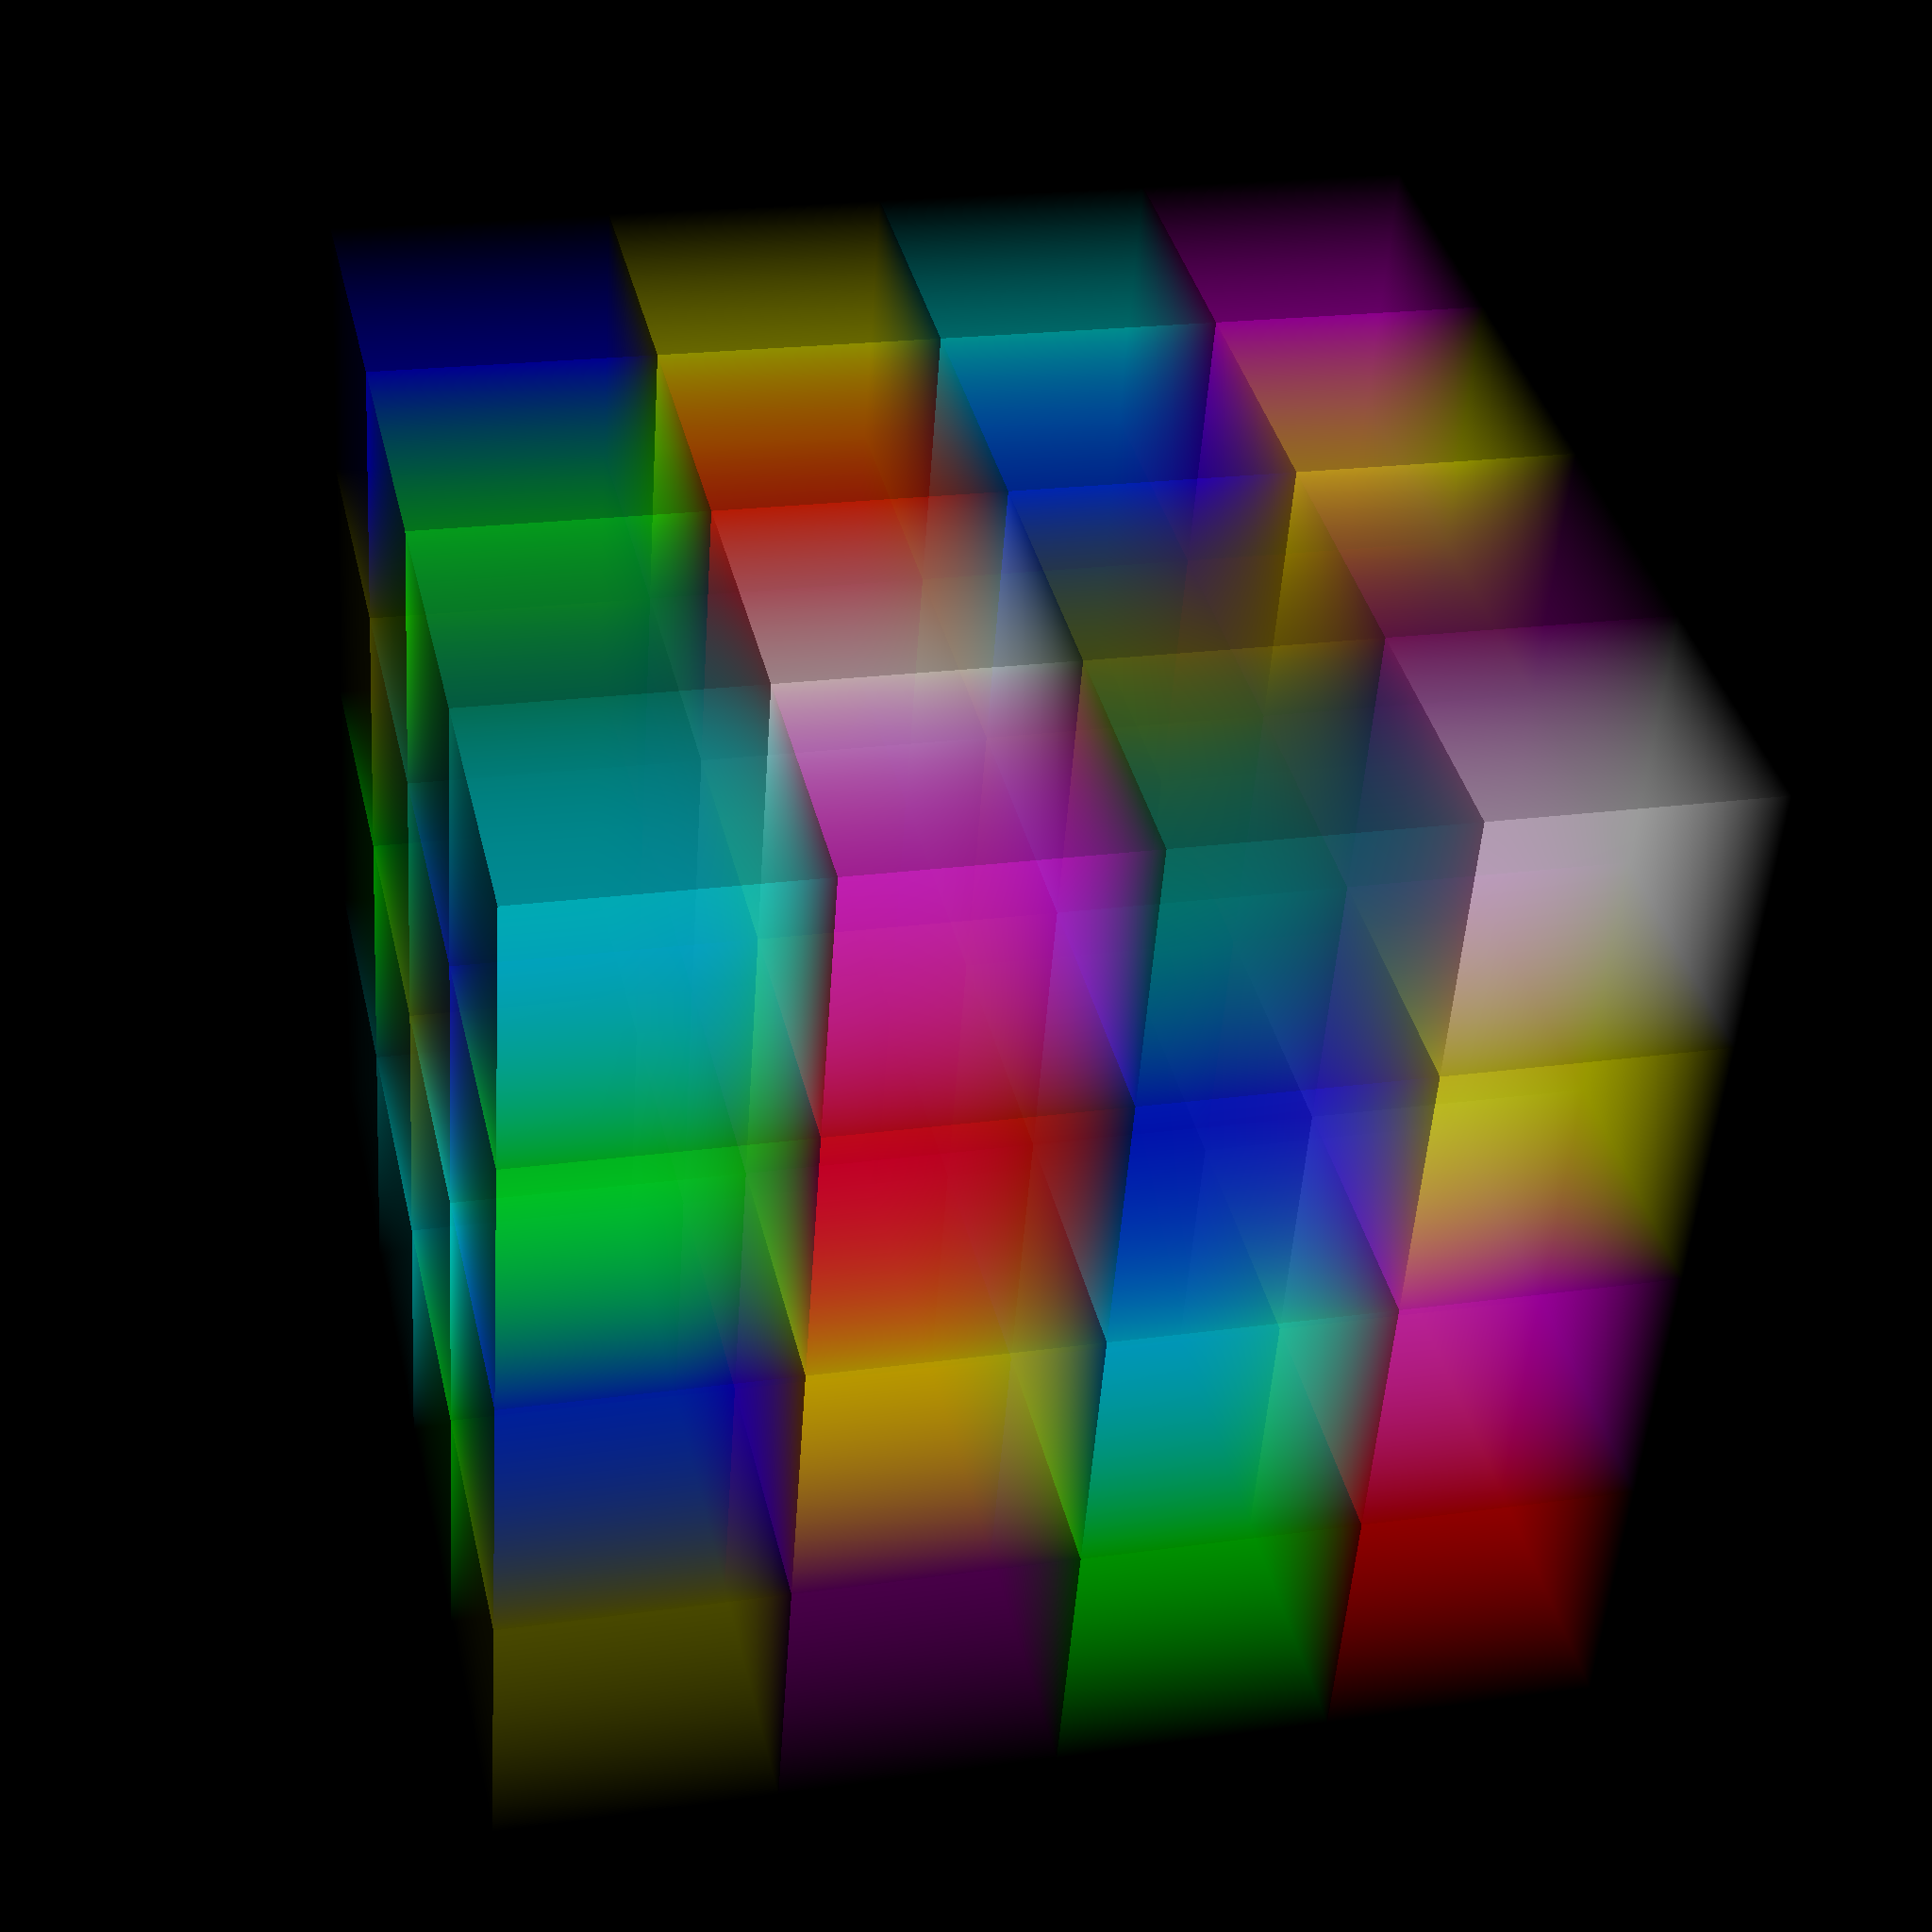
\includegraphics[width=.4\linewidth]{images/TransparentOutput}
  \quad
  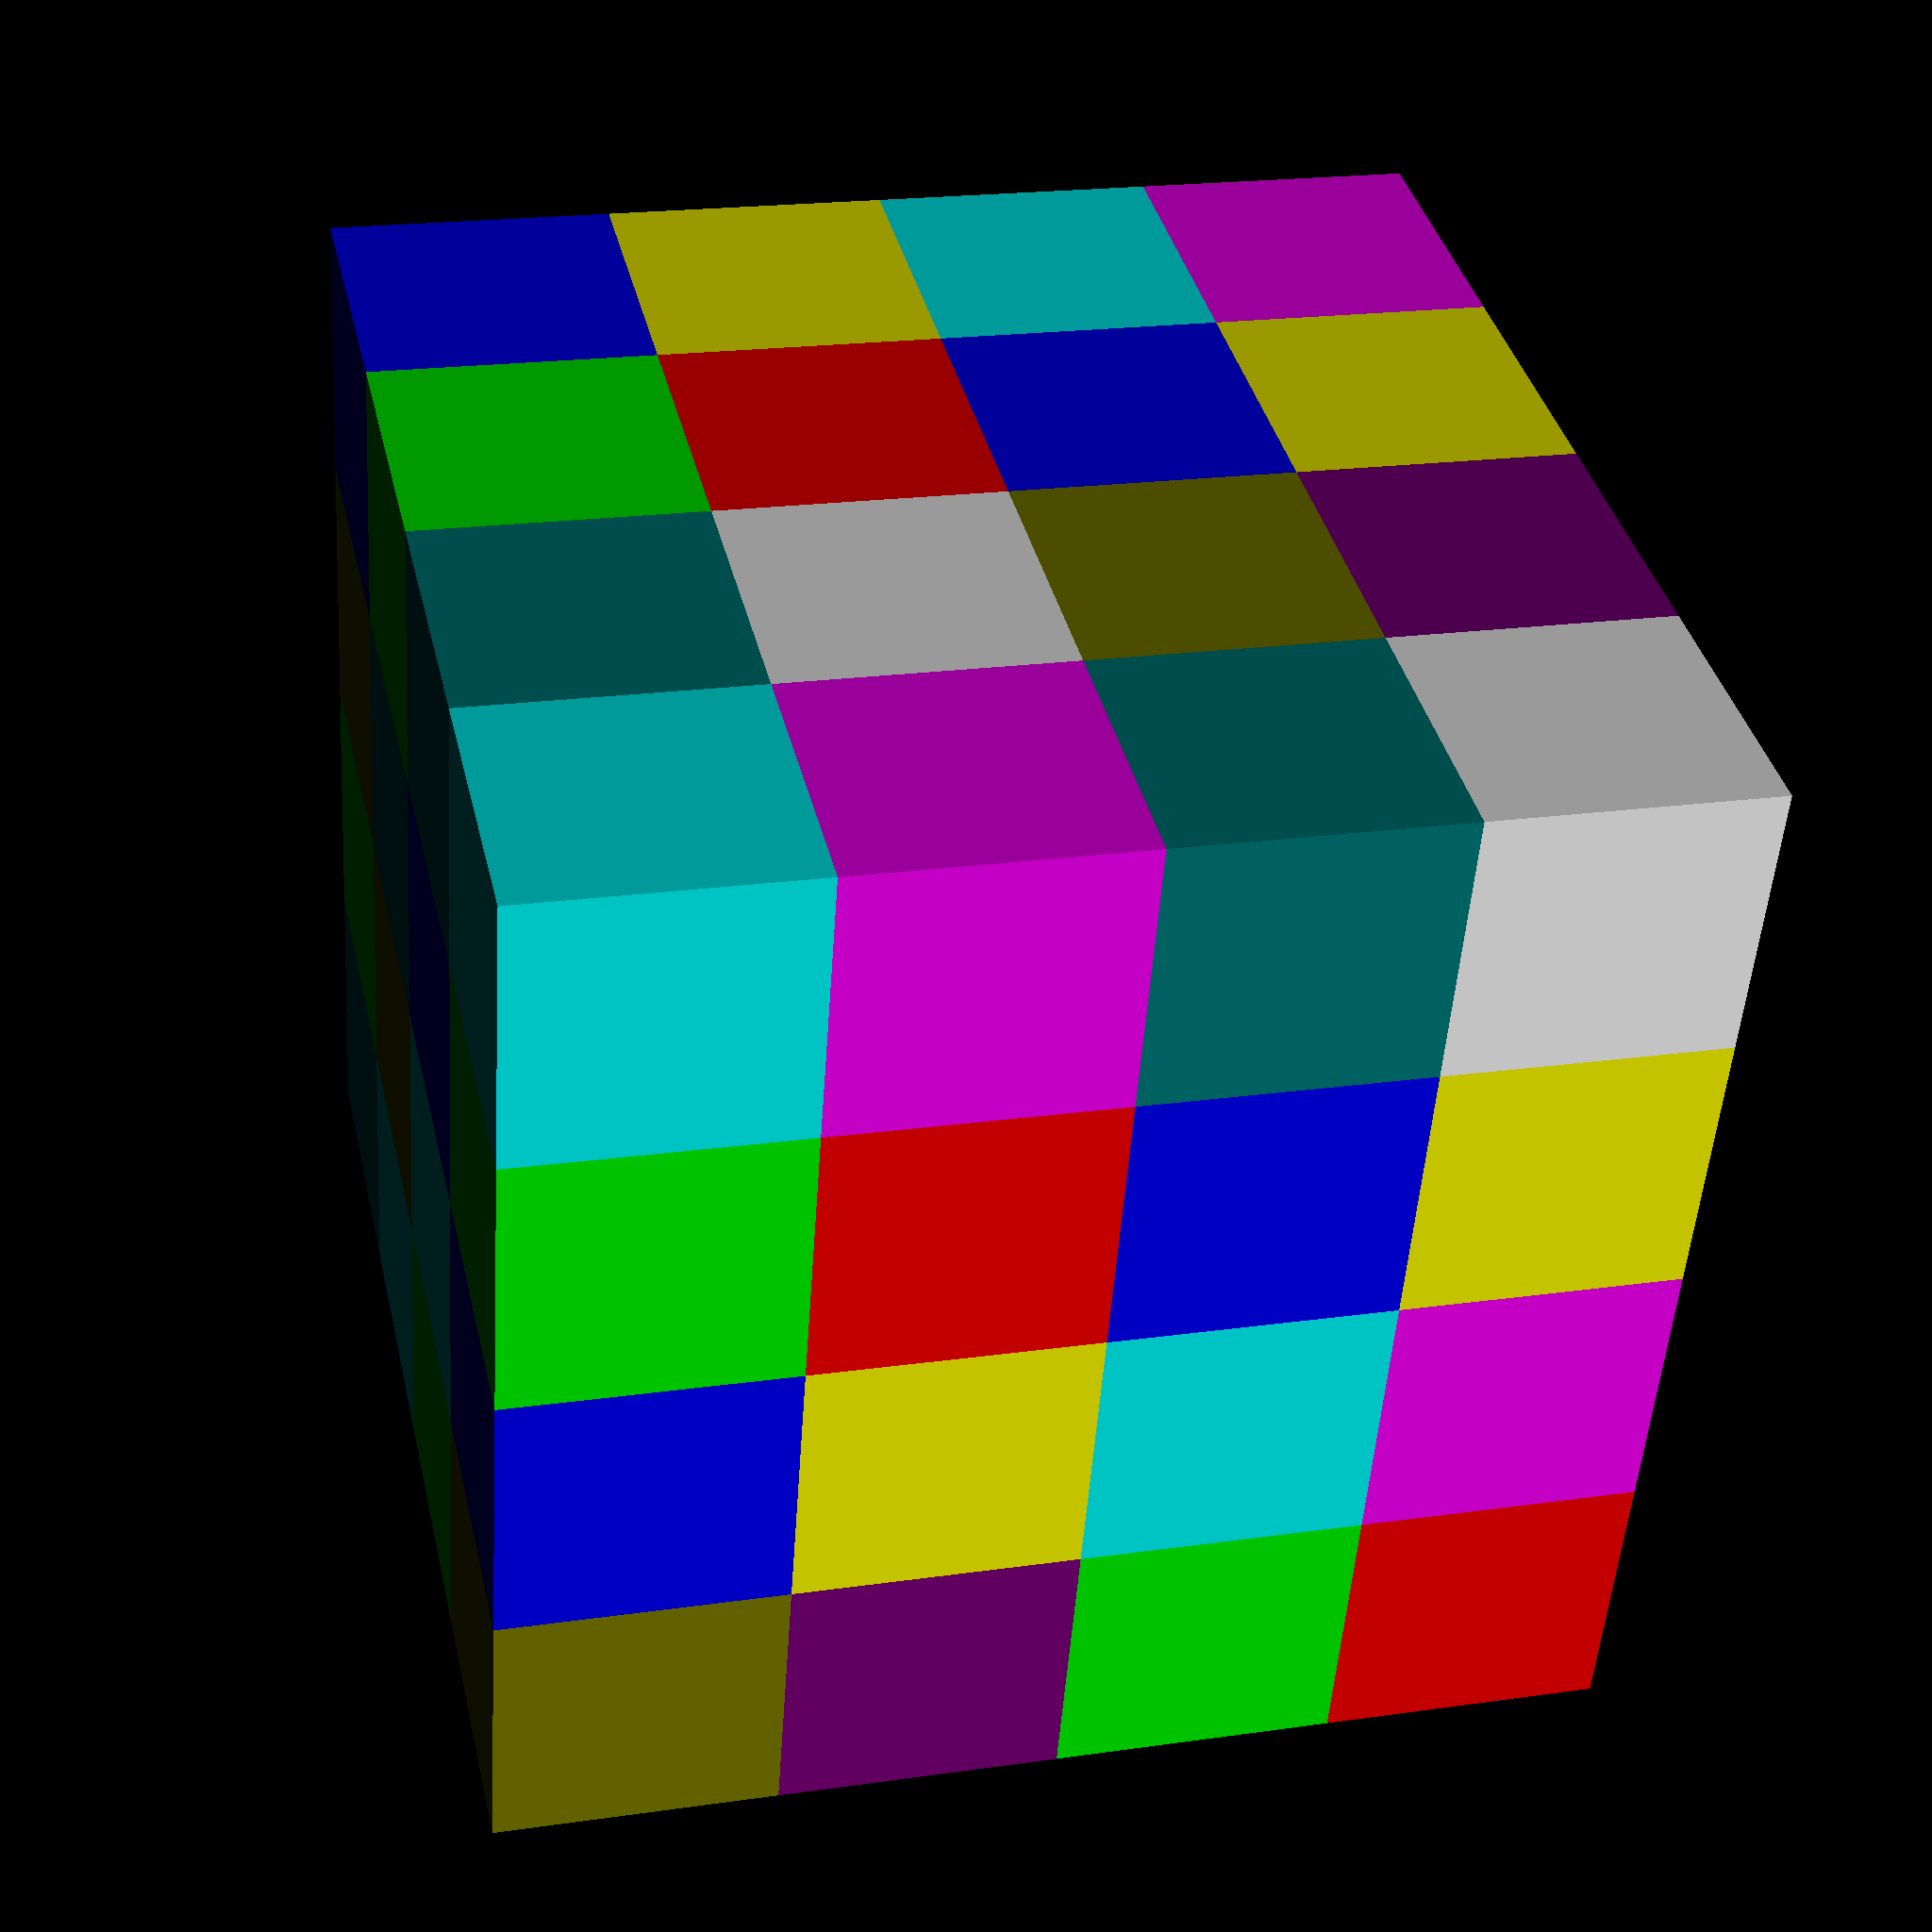
\includegraphics[width=.4\linewidth]{images/OpaqueOutput}
  \caption{Examples of images rendered in our experiments.}
  \label{fig:SimpleTimingOutput}
\end{figure}

Most of the experiments reported in this paper were run on Argonne National
Laboratory's Intrepid Blue Gene/P computer\lcite{BlueGeneP}.  Intrepid
comprises a total of 40,960 nodes, each containing four cores.  Each
experiment was run in one of two modes.  The first mode, \keyterm{Symmetric
Multiprocessing} (SMP), runs a single MPI process on each Intrepid
node.  The intention of the mode is to run multiple threads to use all four
cores, but in our experiments we run a single thread using only one core.
The second mode, \keyterm{Virtual Node} (VN), runs four MPI processes on
each Intrepid node.  It treats each core on the node as a distributed
memory processes even though it is possible to share memory.  Data
transfers amongst the processes within a single node still require explicit
MPI memory passing although the underlying MPI layer bypasses the network
infrastructure in this case.  We consider both running modes because both
are commonly used today and each has differing demands on the underlying
subsystems.

%% Supplemental experiments were run on Sandia National Laboratories' Red Sky
%% computer.  Red Sky comprises a total of 2,279 nodes, each containing dual
%% 2.93 GHz quad core Nehalem X5570 processors (8 cores in all).  Nodes are
%% connected by a QDR InfiniBand network.  All experiments on Red Sky use all
%% eight cores of each node (the equivalent of VN mode on Intrepid).  Red Sky
%% has faster processors than Intrepid but a slower interconnect, which
%% changes the dynamics and optimizations of parallel algorithms run on them.

\section{Compositing Order}
\label{sec:CompositingOrder}

During our integration of radix-k into IceT, we discovered that the
compositing order of incoming images could make a significant performance
difference.  In our initial implementation of radix-k, we got dramatically
different results than those reported by Kendall \etal\scite{Kendall2010}.
Rather than getting improved performance with radix-k, we saw worse
performance.  Deeper inspection revealed that although our radix-k
implementation was properly overlapping communication with compositing
computations, the computations took longer with larger values of $k$.

This increase in compositing time is caused by a change in the order images
are composited together.  The order in which images are composited within a
round is not specified in the original radix-k algorithm; however,
generally images are composited in the order they are received and
accumulated in a single buffer, as demonstrated in
Figure~\ref{fig:CompositeOrder:Accumulative}.  The issue is that composited
images grow with respect to the non-overlapping pixels in each image.
Pixels that do not overlap are simply copied to the output.  In the example
of compositing images for a radix-k round of $k=8$ given in
Figure~\ref{fig:CompositeOrder:Accumulative}, non-overlapping pixels in the
leftmost images are copied up to seven times before the final image is
produced.  In contrast, binary swap performs the equivalent composites in a
tree-like order as shown in Figure~\ref{fig:CompositeOrder:Tree}, and no
pixel needs to be copied more than three times.

\begin{figure}[htbp]
  \centering
  \subfloat[Accumulative Order]{
    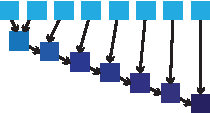
\includegraphics{images/AccumulativeCompositeOrder}
    \label{fig:CompositeOrder:Accumulative}
  }
  \quad
  \subfloat[Tree Order]{
    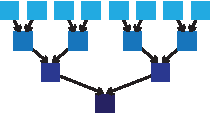
\includegraphics{images/TreeCompositeOrder}
    \label{fig:CompositeOrder:Tree}
  }
  \caption{Two possible orders for compositing eight images.  Boxes
    represent images and arrows indicate how two images are composited
    together to form a third image.}
  \label{fig:CompositeOrder}
\end{figure}

Given this observation, we made two independent improvements to the radix-k
algorithm.  The first improvement speeds-up the compositing computation.
Specifically, run lengths of non-overlapping pixels to be copied are
collected and copied in blocks rather than independently casting and
copying each pixel value one at a time, as was done before.  The second
improvement constrains the compositing to follow the specific tree
composite order.  That is, rather than composite an incoming image whenever
possible, force the compositing to happen in an order like that in
Figure~\ref{fig:CompositeOrder:Tree}.  This constraint may cause radix-k to
wait longer for incoming images, but the overhead is more than compensated
by the improved blending performance.

\begin{figure}[htbp]
  \centering
  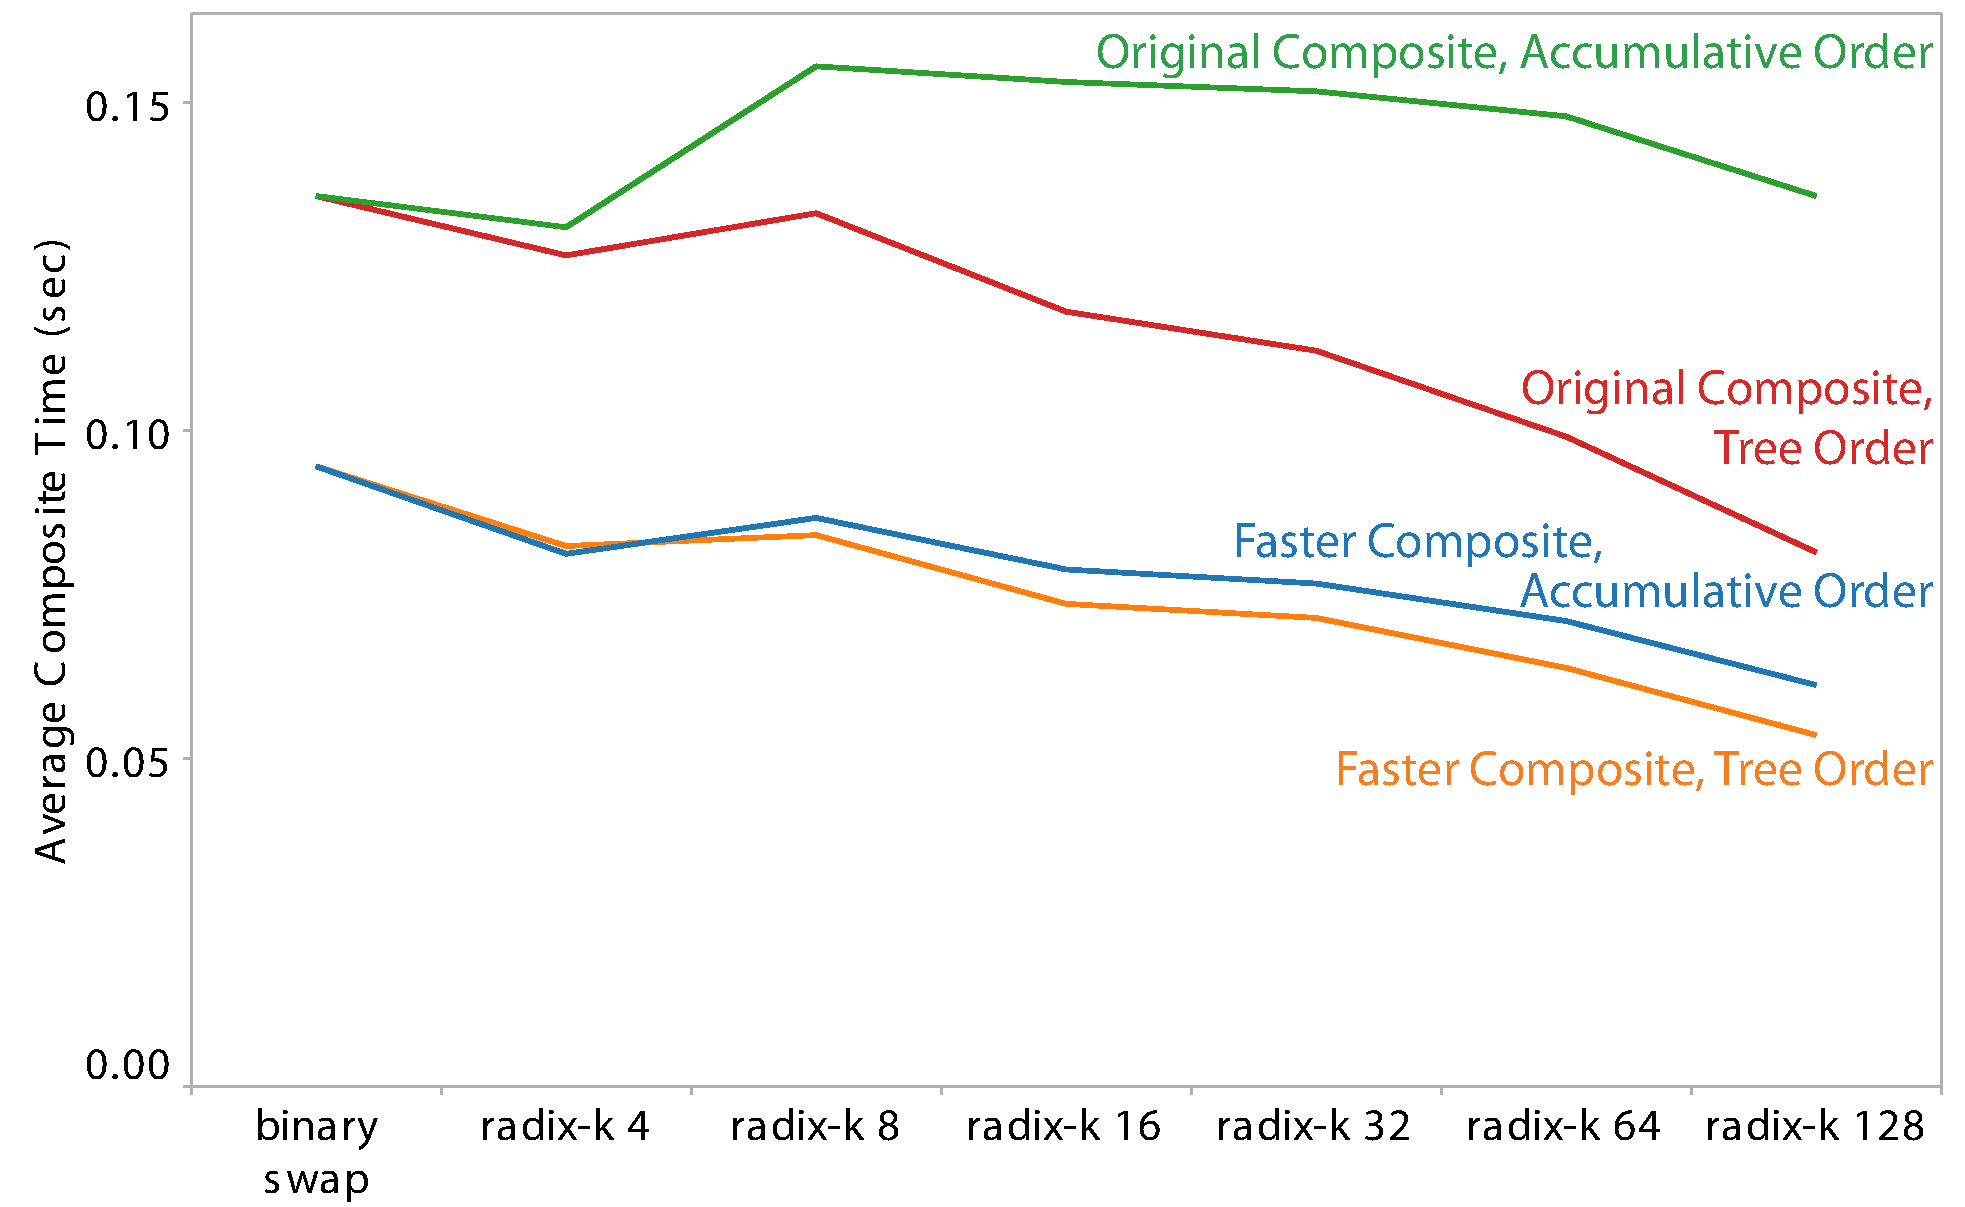
\includegraphics[width=\linewidth]{images/CompositeImprovements0256}
  \caption{Comparative performance of radix-k with improved compositing
    computation and changing the order of compositing.  All runs were
    performed on 256 nodes of Intrepid in SMP mode generating images with
    $2048 \times 2048$ pixels and transparent blending.}
  \label{fig:IceTCompositeImprovements0256}
\end{figure}

\begin{figure}[htbp]
  \centering
  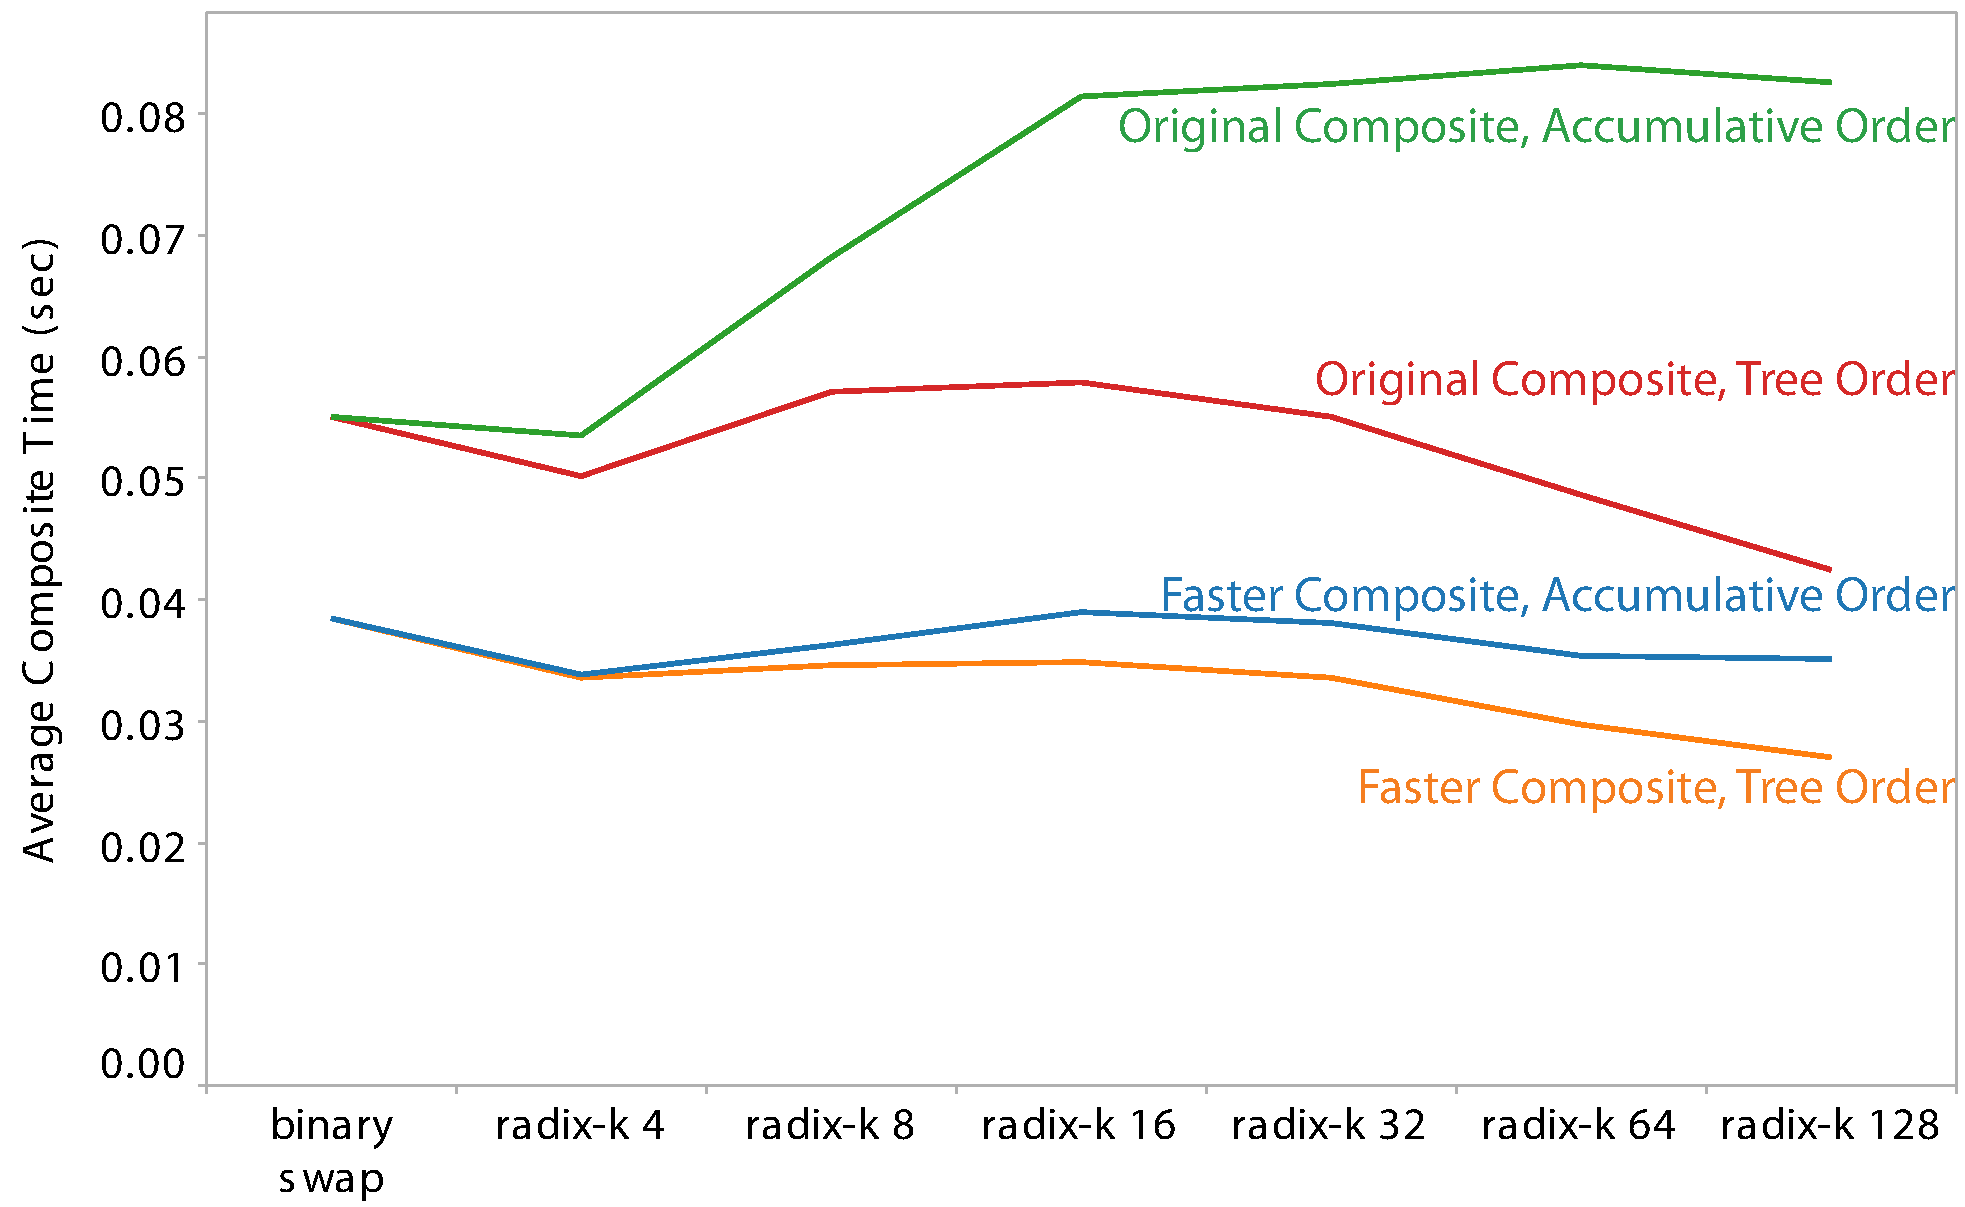
\includegraphics[width=\linewidth]{images/CompositeImprovements2048}
  \caption{Comparative performance of radix-k with improved compositing
    computation and changing the order of compositing.  All runs were
    performed on 2048 nodes of Intrepid in SMP mode generating images with
    $2048 \times 2048$ pixels and transparent blending.}
  \label{fig:IceTCompositeImprovements2048}
\end{figure}

Results of these performance improvements are independently shown in
Figures \ref{fig:IceTCompositeImprovements0256} and
\ref{fig:IceTCompositeImprovements2048}.  The improvements in compositing
computation lower the overall compositing time and reduce the pixel-copying
overhead of larger $k$ values.  The change in composite ordering removes
the extra overhead of pixel-copying and maximizes the performance of larger
$k$ values.

\section{Minimal-Copy Image Interlace}
\label{sec:ImageInterlacing}

The major problem encountered with sparse parallel image compositing is
that it introduces load imbalance, which limits the improvements attained
from compressing images.  A straightforward approach to balance the
compositing work is to interlace the
images\lcite{Molnar1994,Takeuchi2003}.  Interlacing basically shuffles the
pixels in the image such that any region of the image with more compositing
work is divided and distributed amongst the processes.

Interlacing incurs overhead in two places during parallel compositing.  The
first overhead is the shuffling of pixels before any compositing or message
transfers take place.  This overhead tends to be low because it occurs when
images are their most sparse and the work is distributed amongst all the
processes.  The second overhead is the reshuffling after compositing
completes to restore the proper order of the pixels.  This second shuffling
is substantial as it happens when images are at their most full and the
maximum amount of pixels must be copied.  Furthermore, because pixels must
be shuffled over the entire image, this reshuffling must happen after image
data is collected on a single process.  Thus, the reshuffling happens on a
single process while all others remain idle.

Here we provide an interlacing algorithm that completely avoids the needs
for this second reshuffling.  The algorithm is based on the simple
observation that at the completion of either binary swap or radix-k, each
process contains a partition of the final image.  If we arrange our initial
shuffling such that each of the partitions remain a contiguous set of
pixels, then we do not need the final reshuffling at all.

\begin{figure}[htbp]
  \centering
  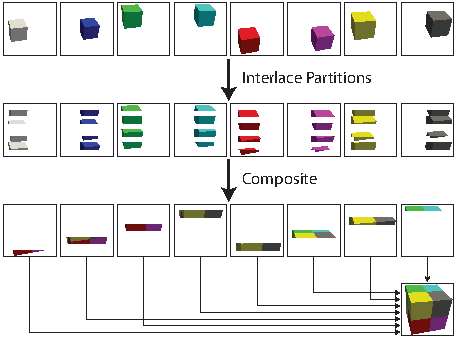
\includegraphics{images/InterlaceDiagram}
  \caption{Pixel shuffling in minimal-copy image interlacing.}
  \label{fig:Interlacing}
\end{figure}

Our minimal-copy image interlacing is demonstrated in
Figure~\ref{fig:Interlacing}.  Rather than picking arbitrary partitions,
such as scan lines, to interlace, our interlacing uses the partitions that
binary swap or radix-k will create anyway.  The partitions are reordered by
reversing the bits of their indices, which creates a van der Corpt sequence
to maximize the distance between adjacent blocks\lcite{LaValle2006}.  The
image with the interlaced block is composited as normal.  Each resulting
image partition is already intact, it is only the implicit offsets that
need to be adjusted.

\begin{figure}[htbp]
  \centering
  \subfloat[256 processes.]{
    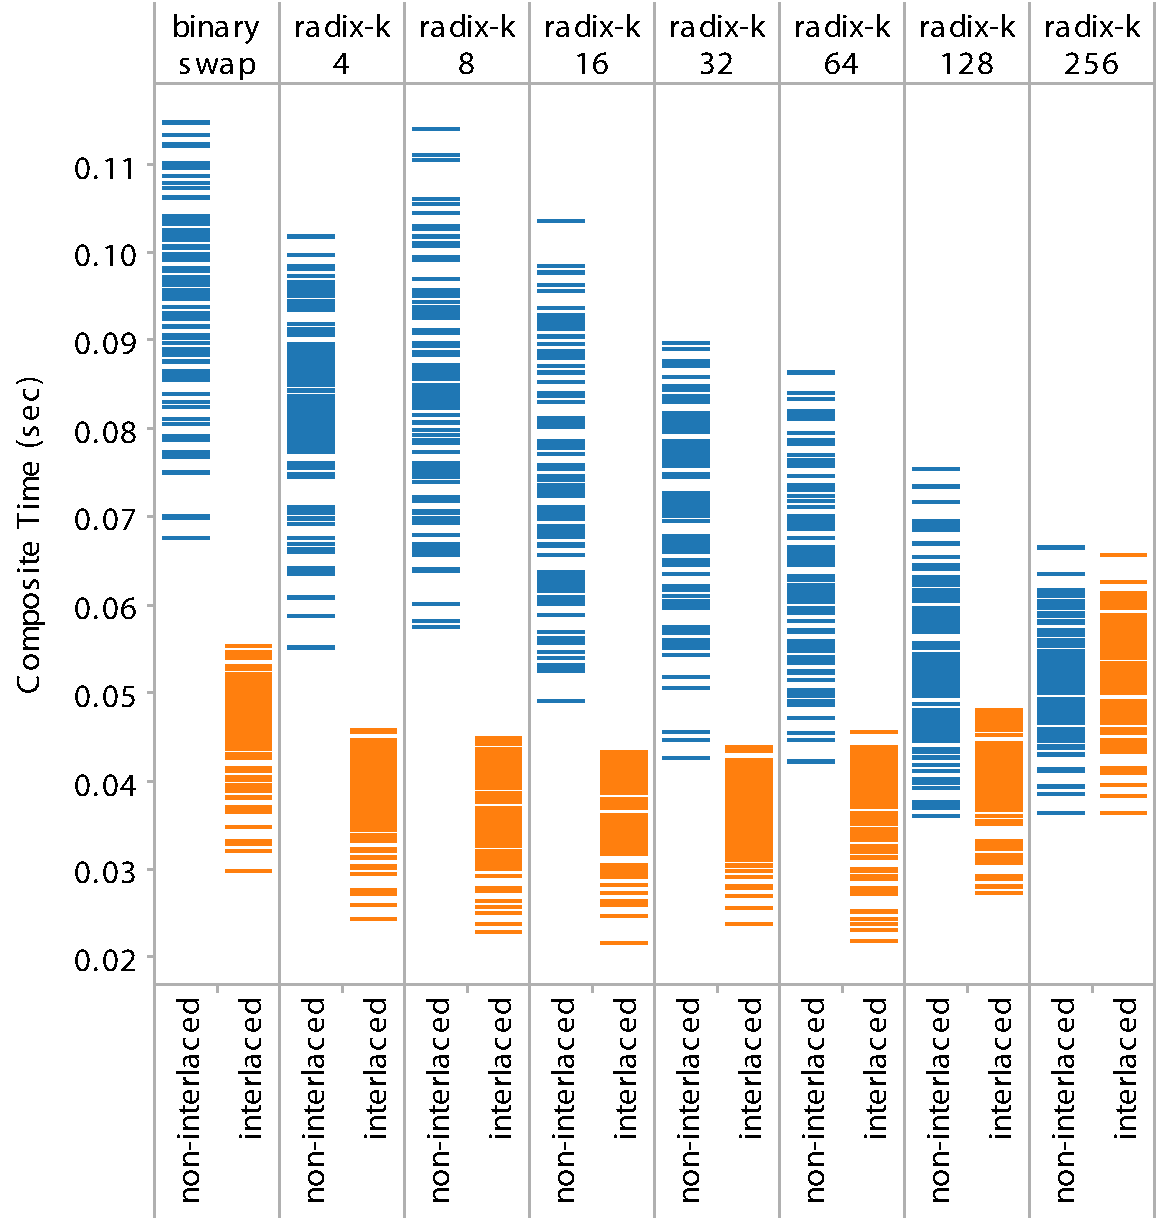
\includegraphics[width=.47\linewidth]{images/Interlace0256}
    \label{fig:InterlacePerformance:256}
  }
  \hfill
  \subfloat[2048 processes.]{
    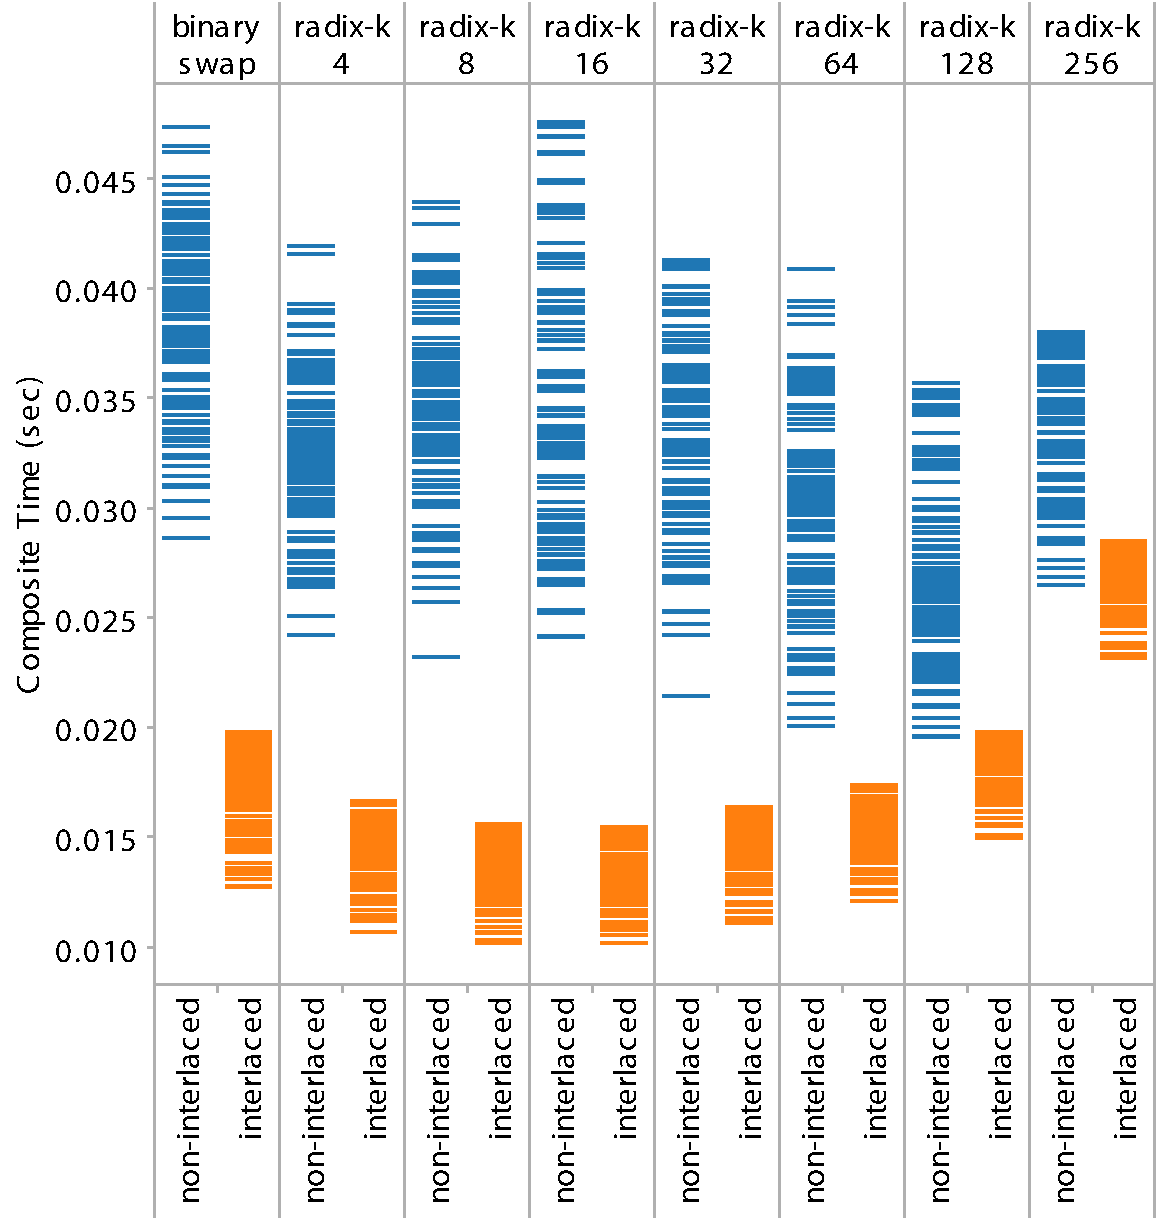
\includegraphics[width=.47\linewidth]{images/Interlace2048}
    \label{fig:InterlacePerformance:1048}
  }
  \caption{Comparative performance of radix-k with and without image
    interlacing.  The composite time for each frame is represented as a
    horizontal line in the plot.  All runs were on Intrepid in SMP mode.}
  \label{fig:InterlacePerformance}
\end{figure}

\begin{figure}[htbp]
  \centering
  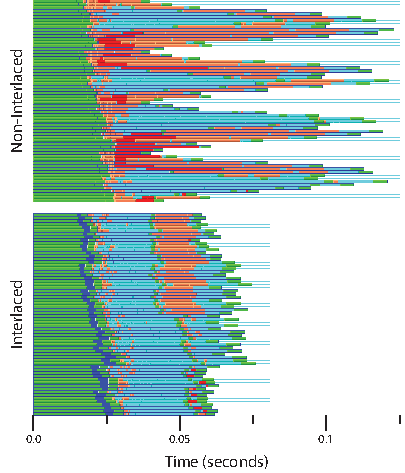
\includegraphics{images/InterlaceJumpshot}
  \caption{Jumpshot logs demonstrating the effect of minimal-copy image
    interlacing.  The cyan color denotes the blending operation whereas the
    salmon and red indicate communication and waiting on messages.  Green
    represents the encoding and splitting of images, and the dark blue is
    the time spent interlacing.}
  \label{fig:InterlaceJumpshot}
\end{figure}

\begin{figure*}
  \begin{codebox}
    \Procname{$\proc{TelescopingComposite}(\id{image}, \id{communicator})$}
    \li $\id{commSize} \leftarrow \proc{size}(\id{image})$
    \li $\id{mainSize} \leftarrow 2^{\lfloor \log_{2} \id{commSize} \rfloor}$
        \Comment Largest power of two less than or equal to \id{commSize}
    \li $\id{remaining} \leftarrow \id{commSize} - \id{mainSize}$
    \li $\id{mainGroup} \leftarrow$ subset of \id{communicator} of size \id{mainSize}
    \li $\id{remainingGroup} \leftarrow$ compliment of \id{mainGroup}
    \li \If $\proc{Rank}(communicator) \in \id{mainGroup}$
    \zi \Then \Comment I belong to the main group.
    \li       $\{ \id{compositedImage}, \id{compositedPartition} \} \leftarrow \proc{BasicComposite}(image, mainGroup)$
    \li       \If $\id{remaining} > 0$
    \zi       \Then \Comment Need to retrieve image
    \li             $\id{sender} \leftarrow$ process in \id{remainingGroup} holding partition corresponding to \id{compositedPartition}
    \label{line:SenderIndexMagic}
    \li             $\id{telescopedImage} \leftarrow \proc{Receive}(\id{sender})$
    \li             $\id{compositedImage} \leftarrow \proc{Blend}(\id{compositedImage}, \id{telescopedImage})$
              \End
    \li       \Return $\{ \id{compositedImage}, \id{compositedPartition} \}$
    \zi \Else \Comment I belong to the remaining group.
    \li       $\{ \id{compositedImage}, \id{compositedPartition} \} \leftarrow \proc{TelescopingComposite}(image, mainGroup)$
    \li       \If $\id{compositedImage} \neq \emptyset$
    \zi       \Then \Comment Still have image data to send.
    \li             $\id{receiverSet} \leftarrow$ all processes in \id{mainGroup} holding a partition corresponding to \id{compositedImage}
    \label{line:ReceiverIndexMagic}
    \li             \For each $\id{receiver} \in \id{receiverSet}$
    \zi             \Do
    \li                  $\id{imagePiece} \leftarrow$ section of \id{compositedImage} matching the image piece in \id{receiver}
    \li                  $\proc{Send}(\id{receiver}, \id{compositedImage})$
                    \End
              \End
    \li       \Return $\{ \emptyset, \emptyset \}$ \Comment Have no image, return nil.
        \End
  \end{codebox}
  \vspace*{-18pt}
  \caption{Algorithm to apply telescoping to an existing parallel image
    compositing function (\proc{BasicComposite}).}
  \label{fig:TelescopingComposite}
\end{figure*}

Figure~\ref{fig:InterlacePerformance} compares the compositing performance
without (blue) and with (orange) image interlacing.  Image interlacing both
reduces the overall time to composite and reduces the variability between
different viewports.  Figure~\ref{fig:InterlaceJumpshot} compares Jumpshot
logs of compositing with and without image interlacing on 64 processes
using radix-k with $k = 16$.  Jumpshot is a profiling tool that shows time
on the horizontal axis and processes as rows on the vertical
axis\lcite{Chan2008}.  With image interlacing, the compositing work is
better balanced and less time is spent waiting for messages.  The overhead
to initially interlace the images is minuscule compared to the time
savings, and the overhead of reshuffling after compositing, as required by
Takeuchi \etal\scite{Takeuchi2003}, or repartitioning during compositing,
as required by Kendall \etal\scite{Kendall2010}.

\section{Telescoping Compositing}
\label{sec:TelescopingCompositing}

A well known problem with binary swap is its inability to deal well with
processor counts that are not a power of two.  A simple and common
technique to apply binary swap to an arbitrary count of processes is
folding.  Folding finds the largest count of processes that is a power of
two and forms a group of that size.  Any process outside of this group (of
which there are always fewer than inside the group) sends its entire image
to one process inside the group where it is blended with the local image.
The processes inside the power-of-two group composite normally while the
remaining processes remain idle.  Yu \etal\scite{23Swap} show that there is
a performance penalty for folding.

2-3 swap\lcite{23Swap} augments binary swap by grouping processes in either
twos or threes in each round rather than exclusively twos.  Because groups
of two and three divide images differently, intermediate steps between
rounds repartition images and send data to ensure that all processes have
image partitions on the same boundaries.  Radix-k also supports process
counts that are not a power of two by forming groups that are any factor of
the process count.  This approach works well if the process count has small
factors, but is inefficient for counts with large factors (as demonstrated
by the results given in Figure~\ref{fig:TelescopeCompositeIntrepidSMP},
which concur with observations of Peterka \etal\scite{Peterka2009} for
direct send).

We provide an alternative algorithm called telescoping for supporting
arbitrary process counts.  Our telescoping algorithm provides a simpler
indexing and partitioning scheme than 2-3 swap and can be applied to most
base parallel compositing algorithms.  We demonstrate telescoping to both
binary swap and radix-k.  Telescoping works similar to folding except
instead of sending images before compositing, images are sent afterward to
minimize idle time.

The \proc{TelescopingComposite} algorithm is listed in
Figure~\ref{fig:TelescopingComposite} and works as follows.  At the onset,
the algorithm finds the largest process subgroup that is a power of two.
Of the remaining processes, it again finds the largest power-of-two
subgroup.  This is repeated until all processes belong to some group that
has a power of two size (where we consider a group of size 1 to be a power
of two equal to $2^0$).  The \proc{TelescopingComposite} procedure finds
groups by recursively calling itself.  The algorithm then independently and
concurrently runs a parallel image compositing (such as binary swap or
radix-k) on each group.

We now assume that each instance of the parallel image compositing results
in an image evenly partitioned amongst all processes.  Most parallel image
compositing algorithms (including binary swap and radix-k) satisfy this
criterion.  To complete the image compositing, processes in the smaller
groups send their partitions to those in the next larger group, starting
with the smallest group.  The second smallest group receives image data
from the smallest, blends this data to its local image data, and sends the
results to the third smallest group.  This continues until the largest
group receives and blends image data from the second largest, at which
point the composite is complete.  Figure~\ref{fig:TelescopeDiagram}
demonstrates the communication pattern of the telescoping algorithm.

\begin{figure}[htbp]
  \centering
  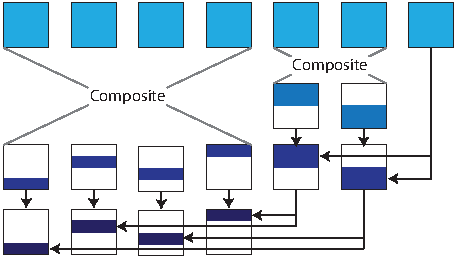
\includegraphics{images/TelescopeDiagram}
  \caption{Augmenting an algorithm to composite on a number of processes
    that is not a power of two.}
  \label{fig:TelescopeDiagram}
\end{figure}

Although the sending of image data across groups happens sequentially (from
smallest to largest), the overhead is minimal.  In binary swap and radix-k,
smaller process groups have fewer rounds and therefore usually finish
earlier.  Thus, by the time the largest groups finish their ``local''
composite, the image data from the next smallest group is usually waiting
in an MPI buffer.

Telescoping is most efficient (and easiest to implement) when the partition
boundaries of a process group of one size align with those of other process
groups.  The image partitioning algorithm in IceT ensures this consistent
partitioning by first computing the regions for partitions of the largest
group and then combining regions for smaller groups.  A second criterion of
running telescoping efficiently is that it is necessary for a smaller group
to know where each partition will be in the larger group and vice versa.
This second criterion is hidden in lines \ref{line:SenderIndexMagic} and
\ref{line:ReceiverIndexMagic} of the \proc{TelescopingComposite} procedure.
As this partition indexing is a necessary part of the implementation of
binary swap or radix-k, determining the same indices for telescoping is
trivial.  It is also trivial to use telescoping with the minimal-copy image
interlacing described in Section~\ref{sec:ImageInterlacing} since the
resulting partitions are the same as those for compositing the largest
process group.

\begin{figure}[tbp]
  \centering
  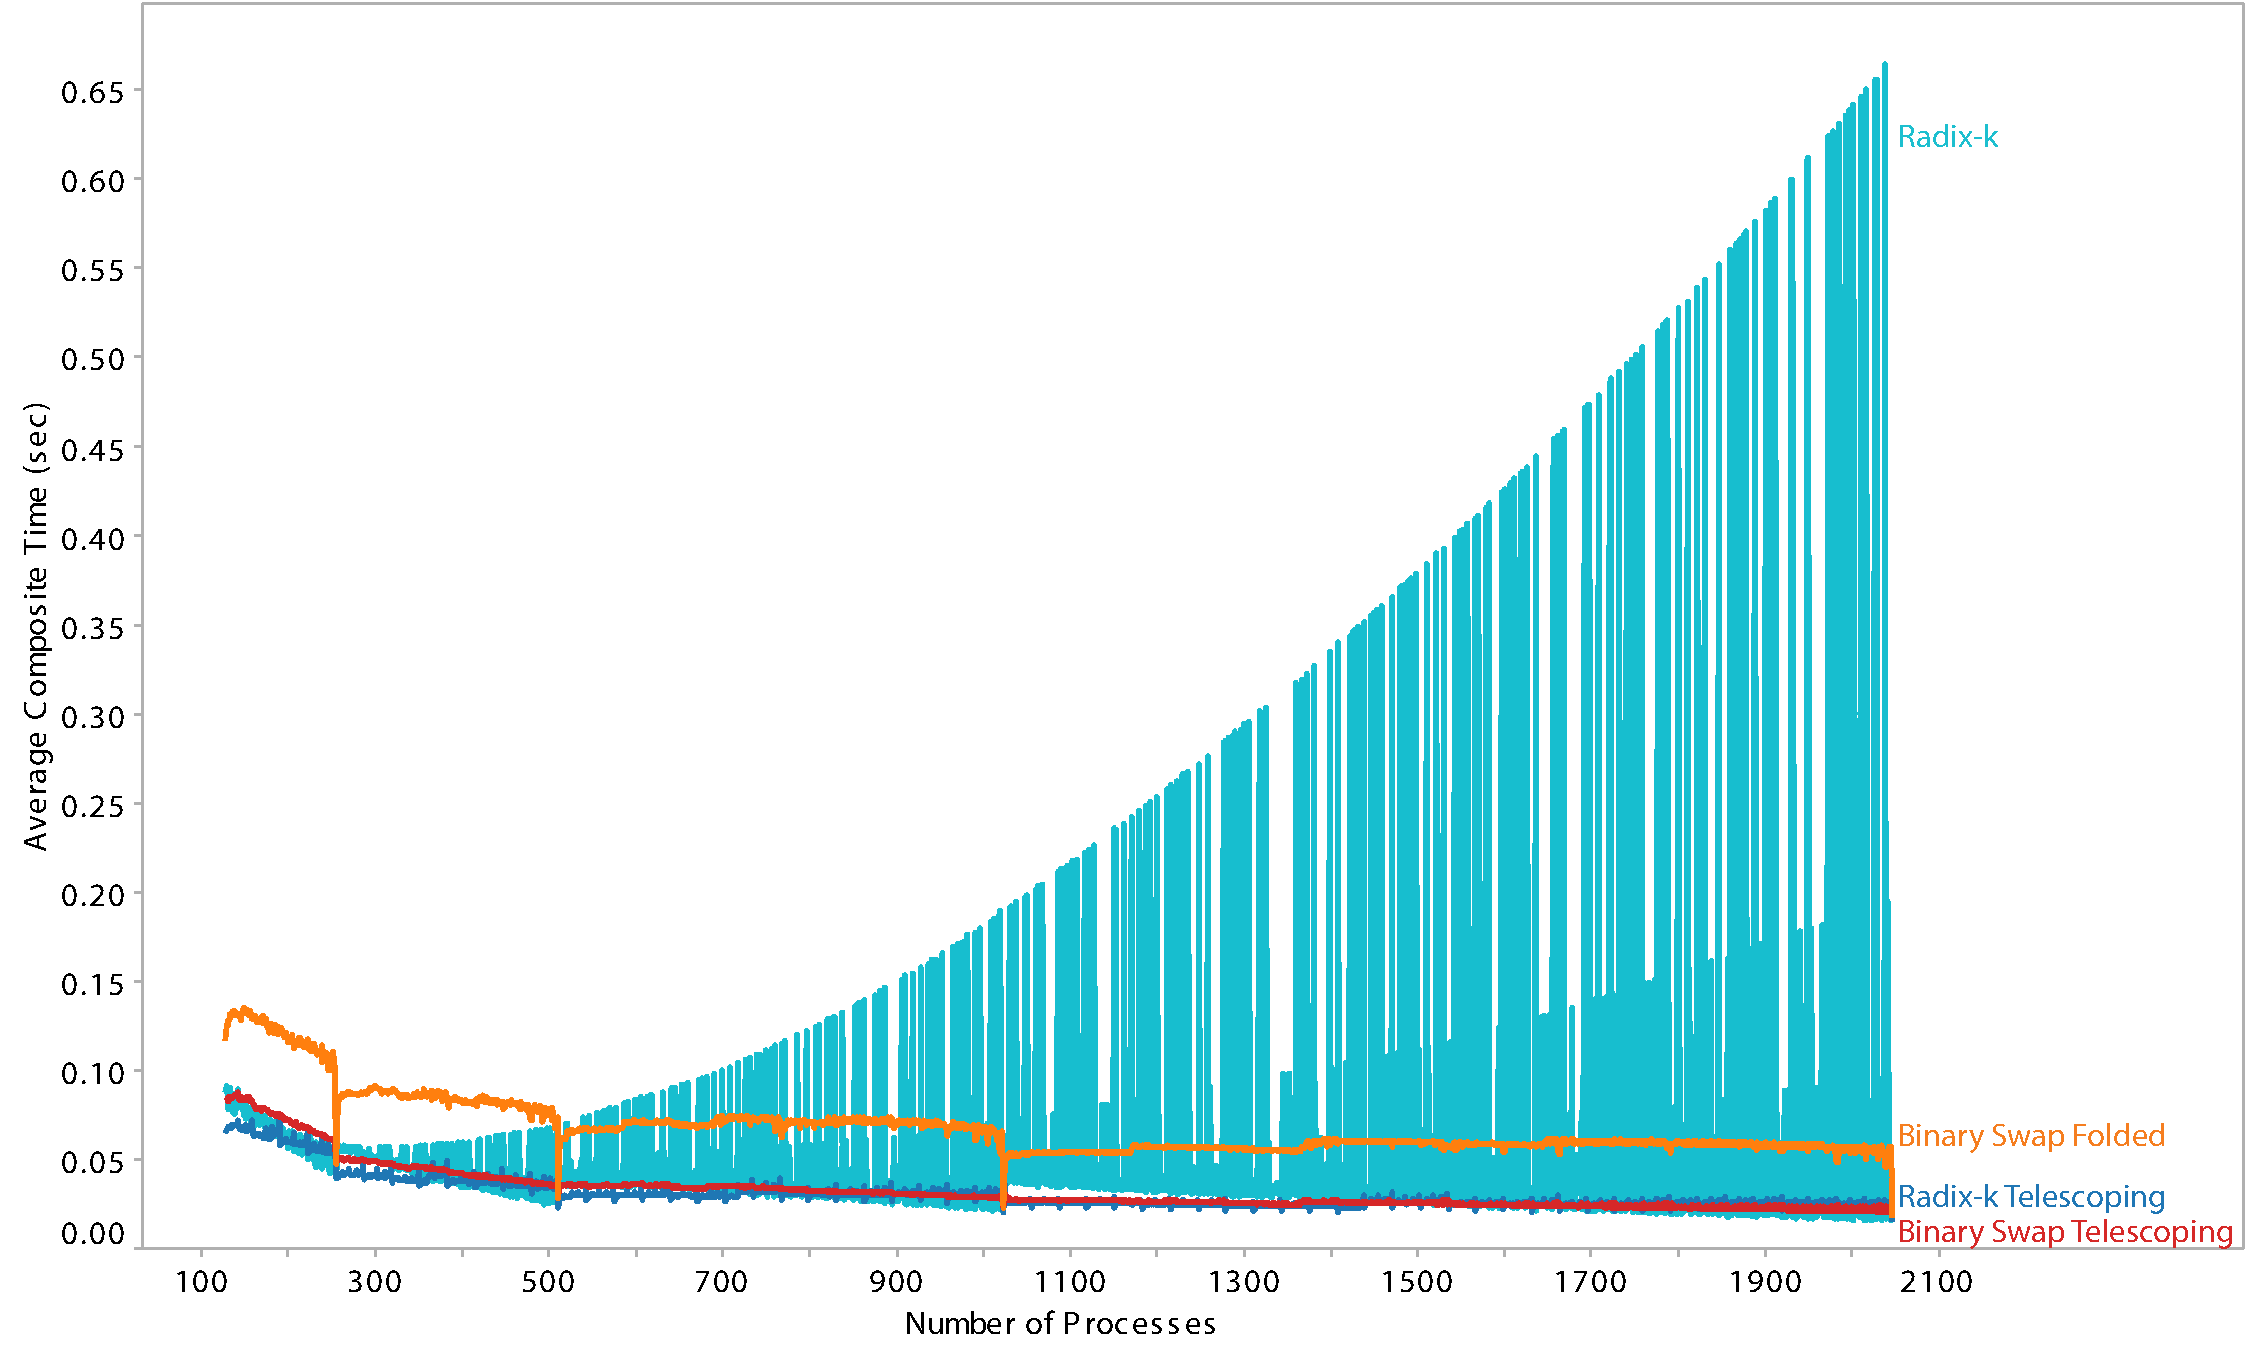
\includegraphics[width=\linewidth]{images/TelescopeCompositeIntrepidSMP}
  \caption{Comparison of telescoping and non-telescoping versions of binary
    swap and radix-k (favoring $k=32$) on Intrepid in SMP mode.}
  \label{fig:TelescopeCompositeIntrepidSMP}
\end{figure}

\begin{figure}[tbp]
  \centering
  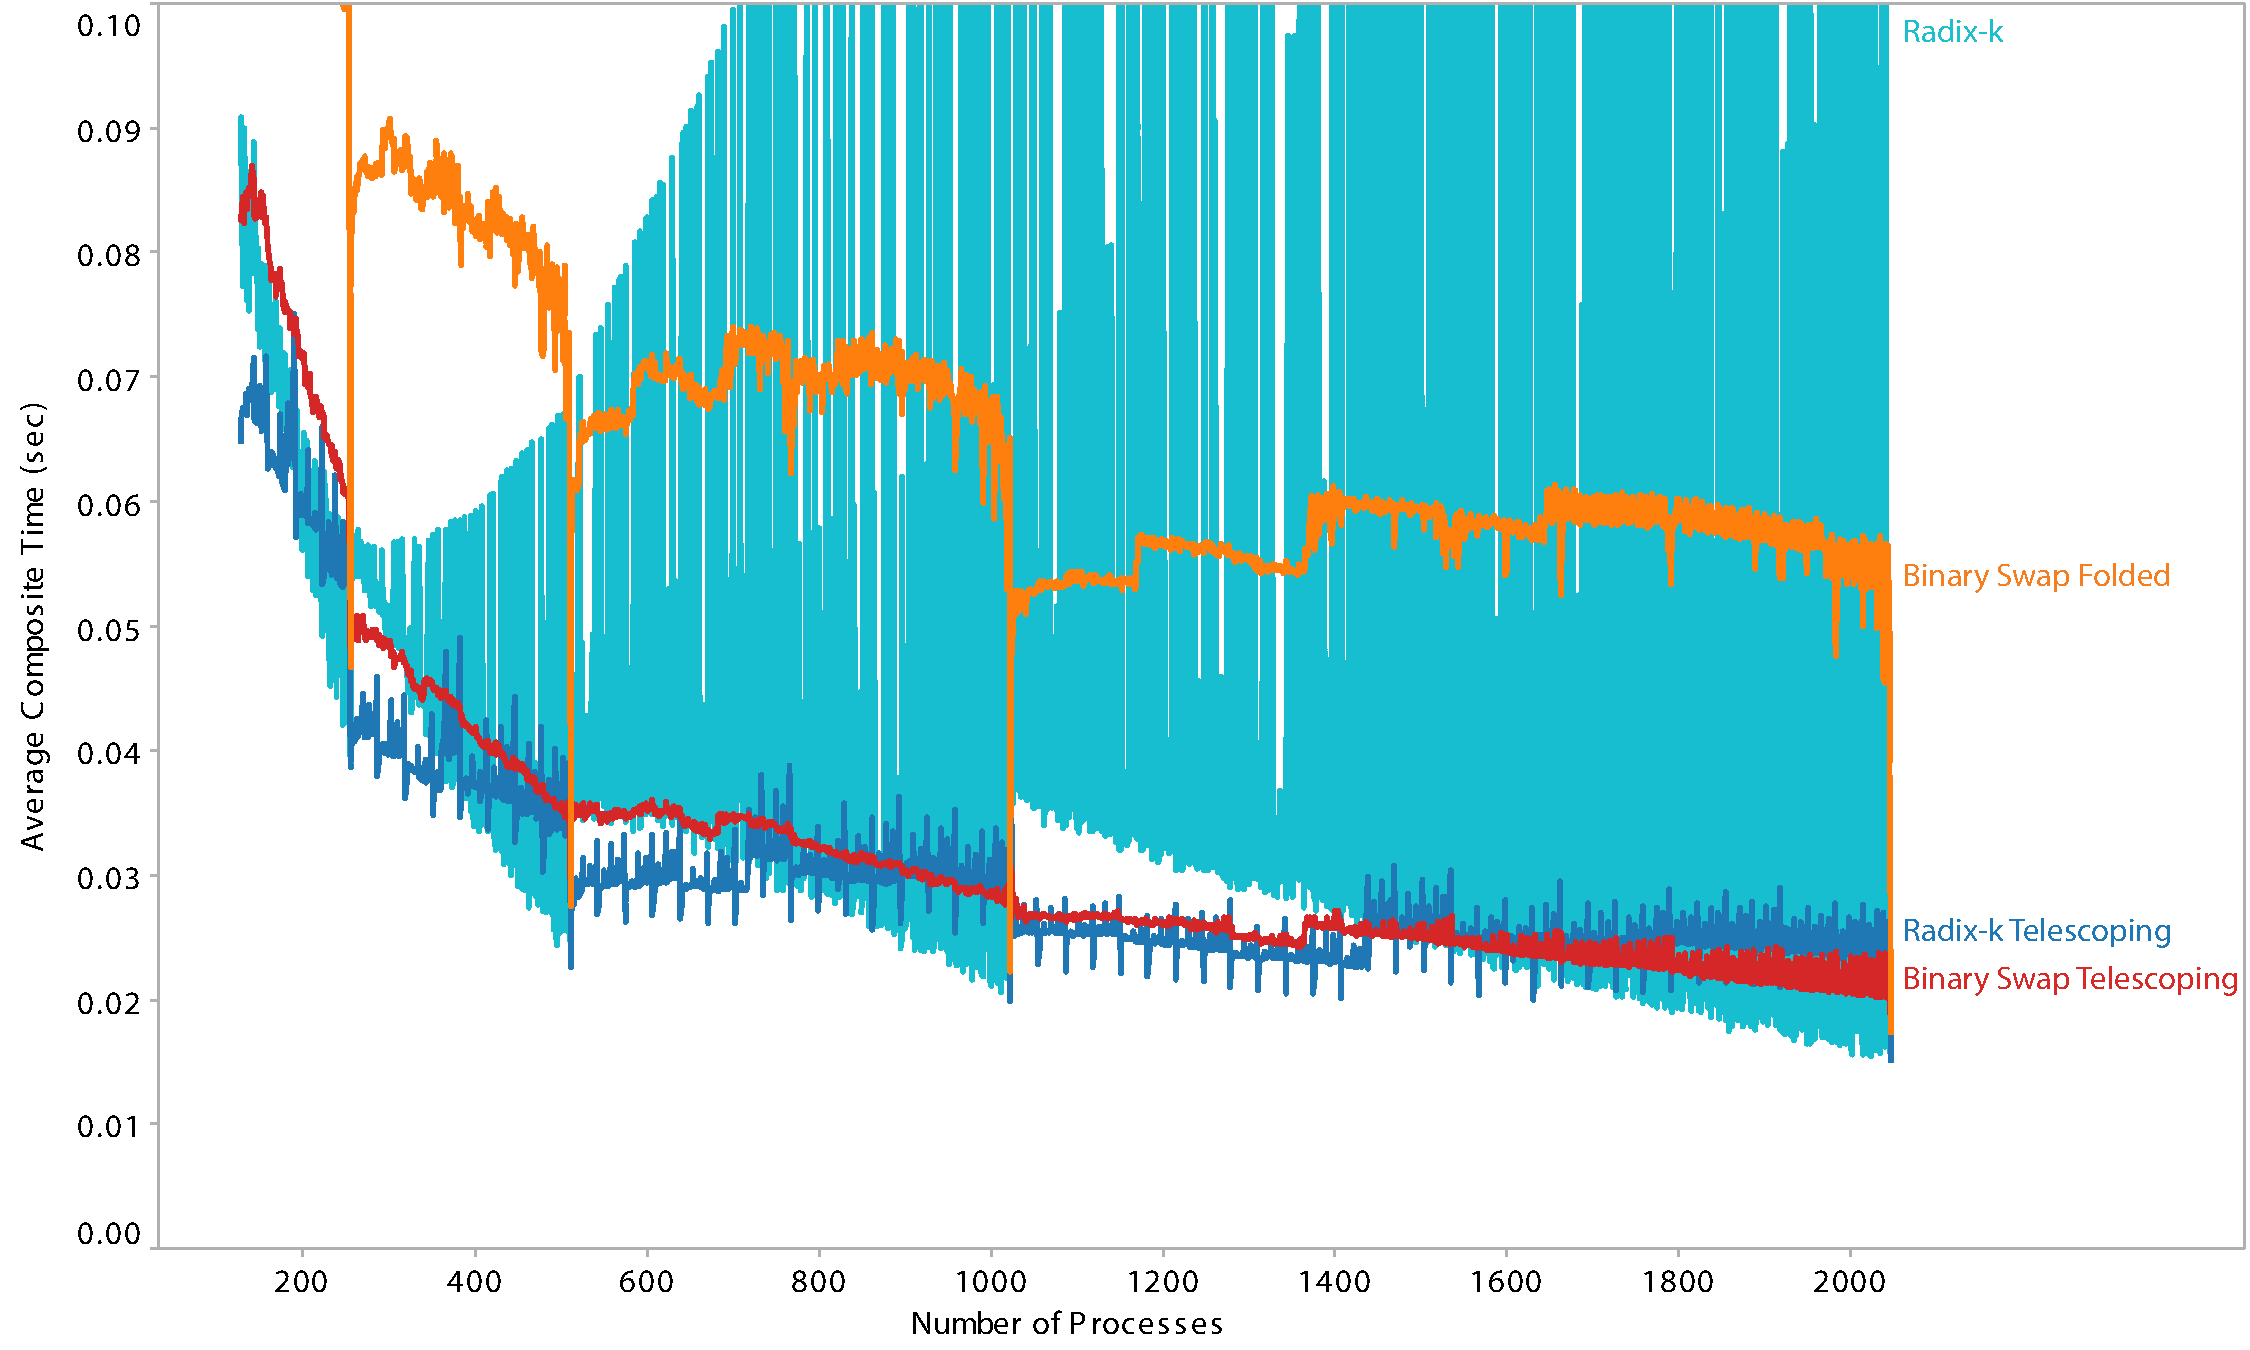
\includegraphics[width=\linewidth]{images/TelescopeCompositeIntrepidSMPZoomed}
  \caption{Comparison of telescoping and non-telescoping versions of binary
    swap and radix-k (favoring $k=32$) on Intrepid in SMP mode.  The
    vertical axis is scaled to see detail in the telescoping algorithms.}
  \label{fig:TelescopeCompositeIntrepidSMPZoomed}
\end{figure}

Figures \ref{fig:TelescopeCompositeIntrepidSMP} and
\ref{fig:TelescopeCompositeIntrepidSMPZoomed} report the performance of
binary swap and radix-k on Intrepid with and without telescoping.  Unlike
the other data given in this paper, these measurements come from the
averaging of 10 frames rather than 100 due to the large number of
measurements we took.  Figure~\ref{fig:TelescopeCompositeIntrepidSMP}
demonstrates that the original radix-k performs well for some process
counts but poorly for others.
Figure~\ref{fig:TelescopeCompositeIntrepidSMPZoomed} shows an overhead for
folding binary swap analogous to that reported by Yu \etal\scite{23Swap}.
Telescoping makes both algorithms perform reasonably consistent for all
process counts.

\begin{figure}[tbp]
  \centering
  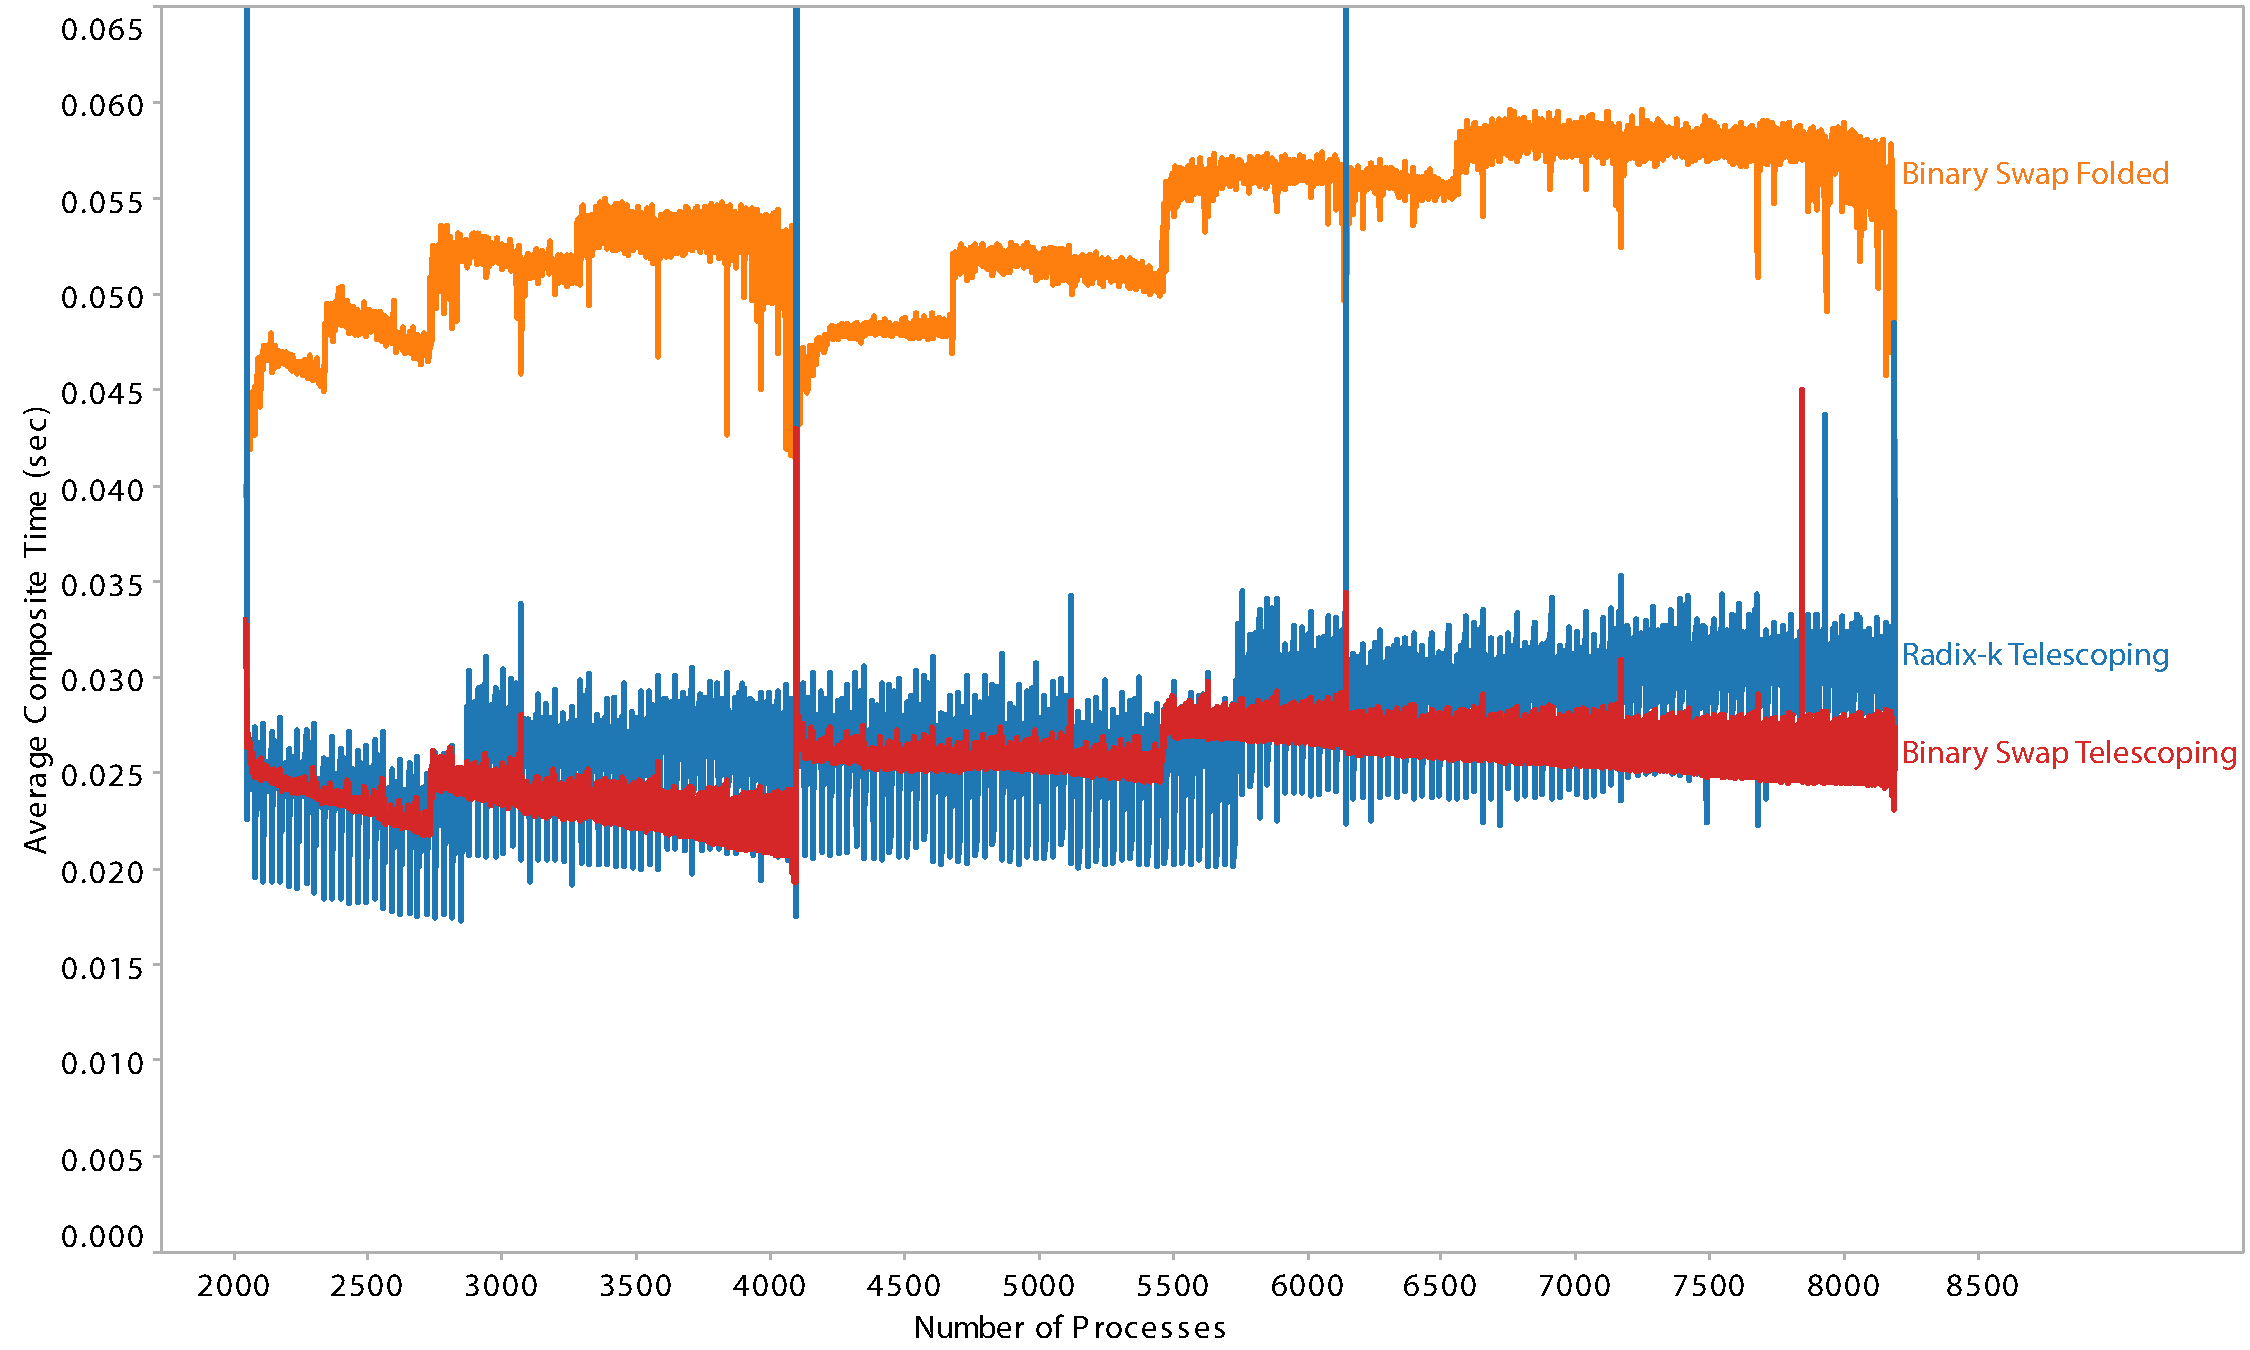
\includegraphics[width=\linewidth]{images/TelescopeCompositeIntrepidVN}
  \caption{Comparison of telescoping and non-telescoping versions of binary
    swap and telescoping version of radix-k (favoring $k=32$) on Intrepid
    in VN mode.}
  \label{fig:TelescopeCompositeIntrepidVN}
\end{figure}

Figure~\ref{fig:TelescopeCompositeIntrepidVN} shows the data for the same
experiment scheduled on Intrepid in VN mode to larger process counts (and
again using 10 frames per measurement).  Values for radix-k without
telescoping are not shown because the frame times are too long to measure
in the amount of processor time we have available.  We did, however, record
times for the largest process counts where we expect the worst behavior.
Our longest average measurement with unaltered radix-k is 12.88 seconds per
frame for 8191 processes (which is, unsurprisingly, the largest prime
number of processes for which we ran).  The same compositing using the
telescoping version of radix-k took only about 0.05 seconds per frame.

We also note some telescoping radix-k measurements in VN mode that are
anomalous compared to other process counts (although consistent for all
frames of that run).  Note the blue spikes in
Figure~\ref{fig:TelescopeCompositeIntrepidVN}.  The largest such spike is
0.55 seconds per frame at 4097 processes.  We are not sure why these spikes
occur, but we observe that they happen when a small process group has to
send images to a much larger process group.  Since these spikes only occur
with radix-k and in VN mode, we suspect that this telescoping communication
is happening at the same time as the larger group's radix-k communication,
and the two interfere with each other.  This is explained by the fact that
in VN mode four processes share a single network interface controller,
which must serialize incoming and outgoing messages.

\section{Image Collection}
\label{sec:ImageCollection}

As previously mentioned, parallel compositing algorithms finish with image
data partitioned amongst the processes.  Although the compositing is
technically finished at this point, it is of little practical use if it is
split into thousands of pieces and distributed across nodes.  Real use
cases require the images to be collected in some way.  For example,
ParaView collects the image to the root node and then sends it over a
socket to a GUI on the user's client desktop\lcite{Cedilnik2006}.

\begin{figure}[htbp]
  \centering
  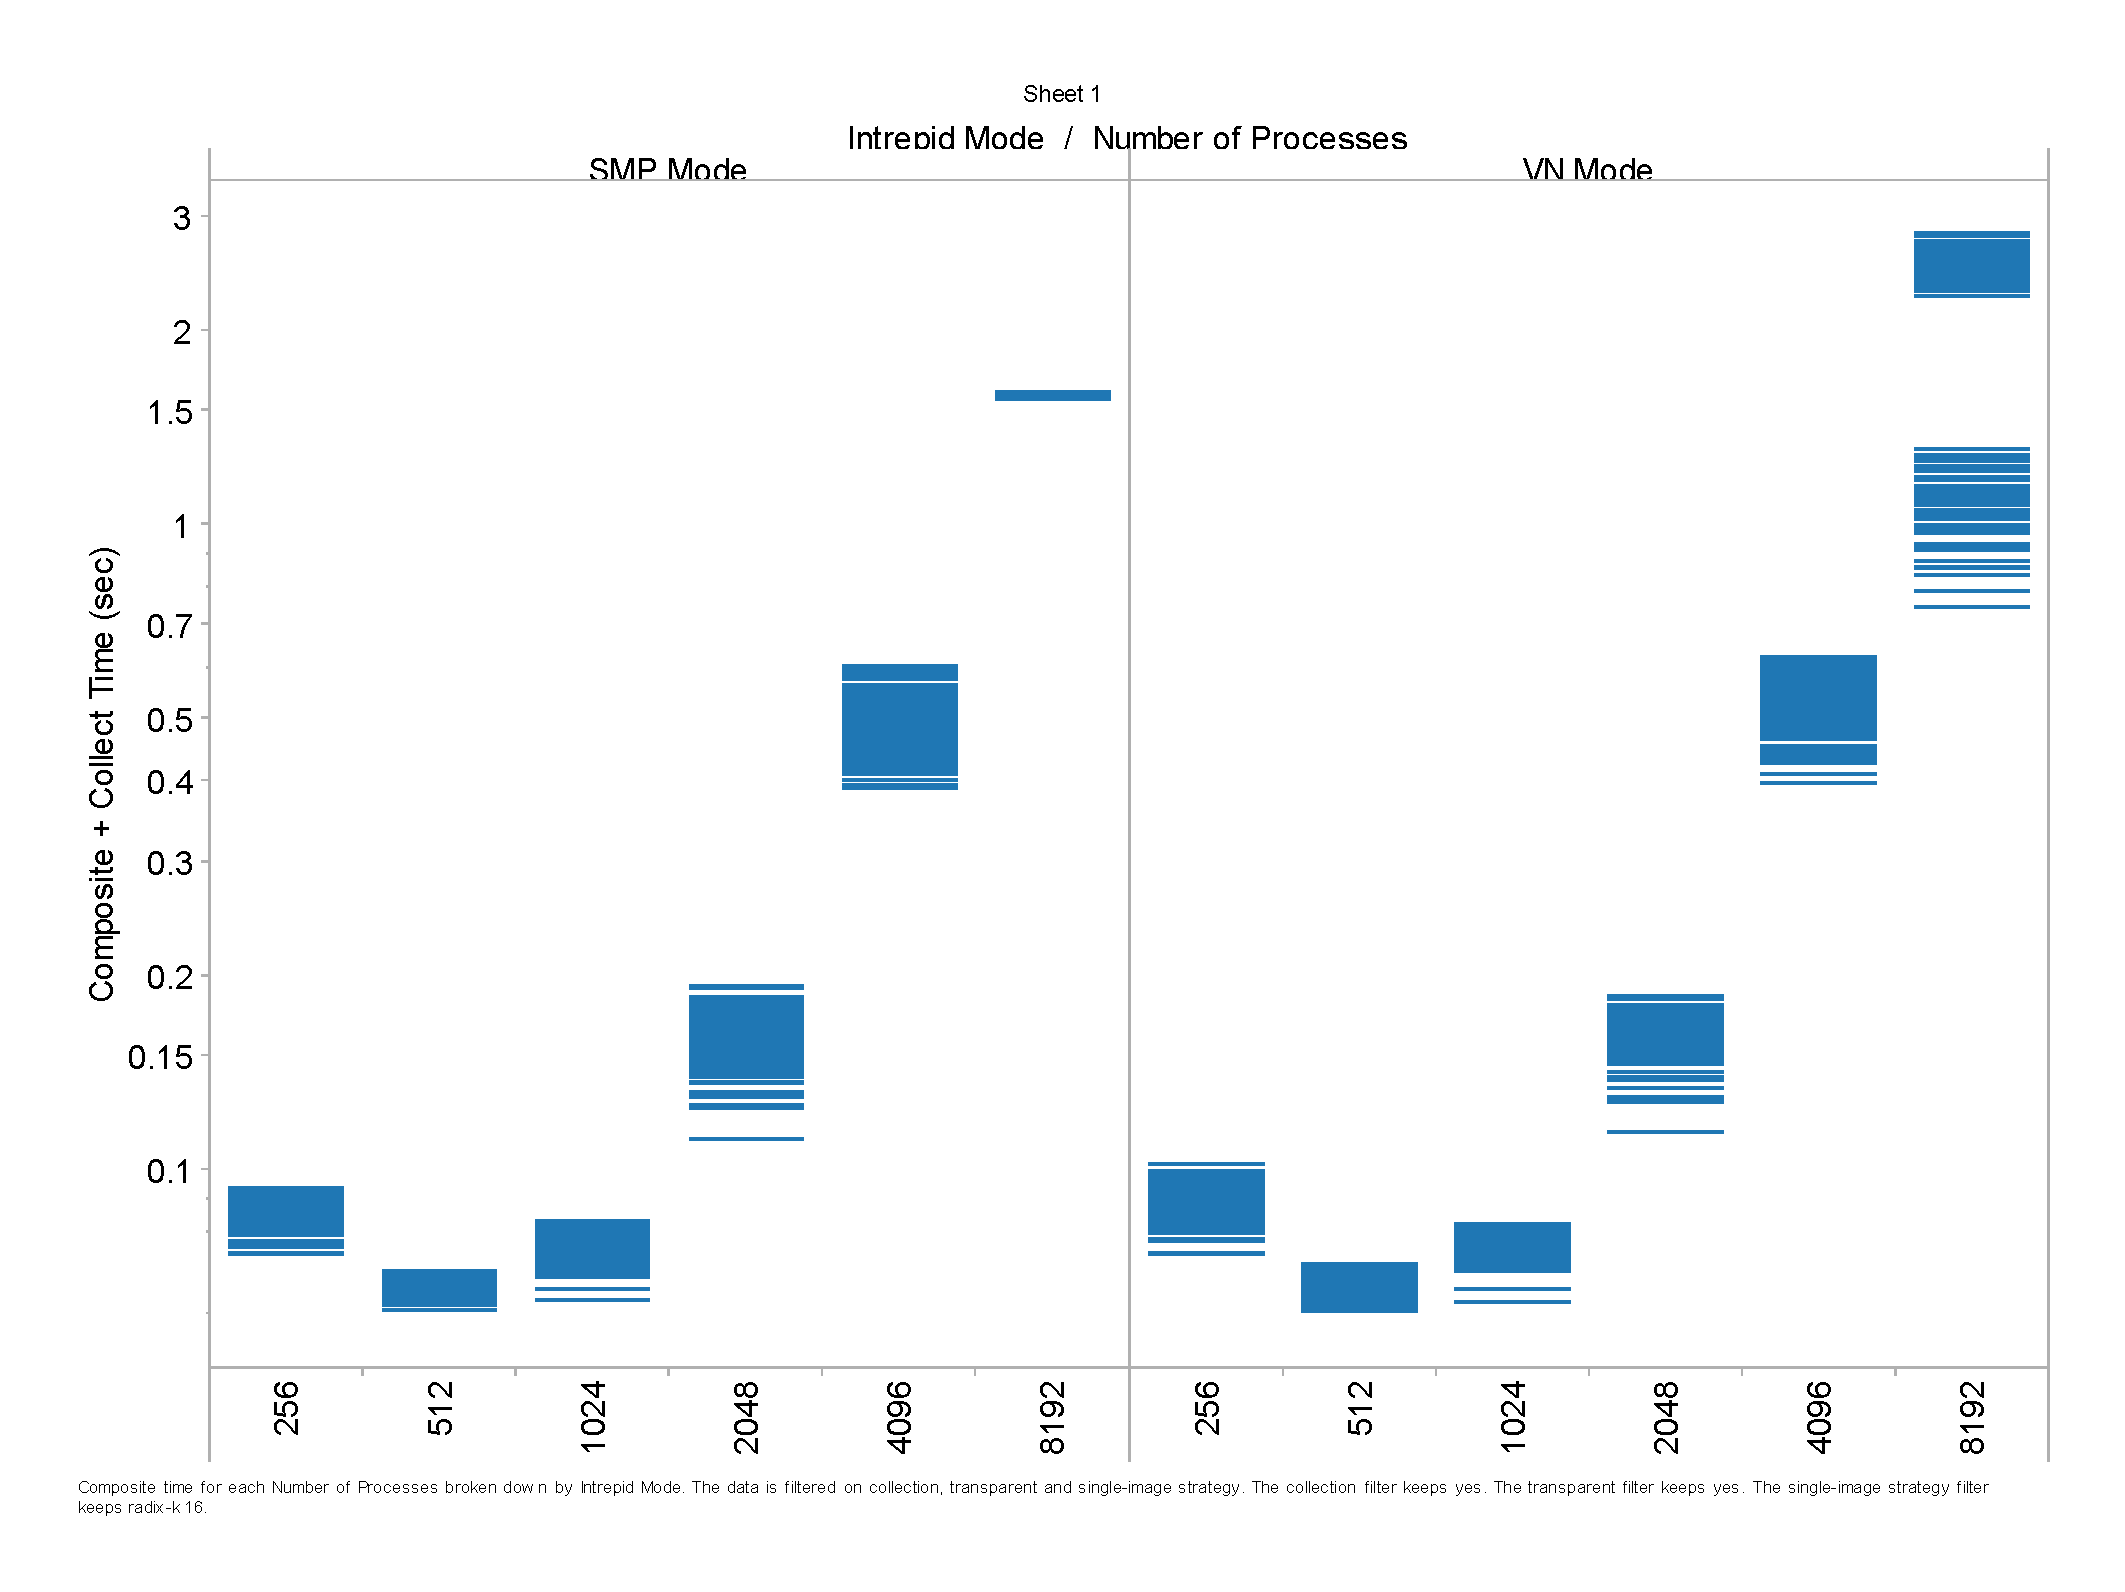
\includegraphics[width=\linewidth]{images/PartitionCollectIntrepidFull}
  \caption{Compositing times on Intrepid when considering time to collect
    image fragments into single image.  All times are given for binary
    swap.}
  \label{fig:PartitionCollectFull}
\end{figure}

Because the collection of the image is so important in practice, it is
proper to also measure its effect when scaling the image compositing
algorithm.  Figure~\ref{fig:PartitionCollectFull} compares compositing
times with and without image collection using an MPI\_Gatherv operation.
Although the numbers given here are only given for binary swap, the
variance between versions is minor compared to the overhead of collection.

Clearly the MPI\_Gatherv collect is not scaling as well with respect to the
rest of the compositing algorithm.  To make the collection more efficient,
we propose limiting the number of partitions created in the parallel
compositing algorithm with a simple change to the binary swap and radix-k
algorithms.  The algorithms proceed in rounds as before.  As long as the
total number of partitions created remains under a specified threshold,
images are split and swapped as normal.  However, when this threshold of
partitions is reached, images are no longer split.  Instead, one process
collects all the image data from other processes in the group.  The
collection process continues while the other processes drop out.
Figure~\ref{fig:CollectRounds} demonstrates two rounds of binary swap with
one of the rounds collecting to reduce the number of partitions.
Collection in radix-k works the same except that $k$ images are collected.

\begin{figure}[htbp]
  \centering
  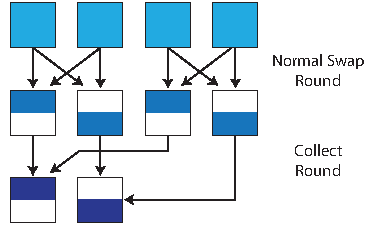
\includegraphics{images/CollectRounds}
  \caption{Reducing the number of partitions created by four process in
    binary swap to two partitions by collecting in the second round.}
  \label{fig:CollectRounds}
\end{figure}

Because this change causes processes to sit idle, it makes the compositing
less efficient but potentially makes the collection more efficient.
Collecting rather than splitting images is only useful to the point where
the improvements in collection outweigh the added inefficiencies in
compositing.  We should also note that limiting the number of partitions
creates limits the number of partitions used in the minimal-copy image
interlacing described in Section~\ref{sec:ImageInterlacing}, but since our
reduced image partitions only contain a few scan lines, the effect is
minimal.  Limiting the number of partitions also changes the indexing in
the \proc{TelescopingComposite} algorithm (listed in
Figure~\ref{fig:TelescopingComposite}) and adds a condition for when the
internally called \proc{BasicComposite} returns a null image.

\begin{figure}[htbp]
  \centering
  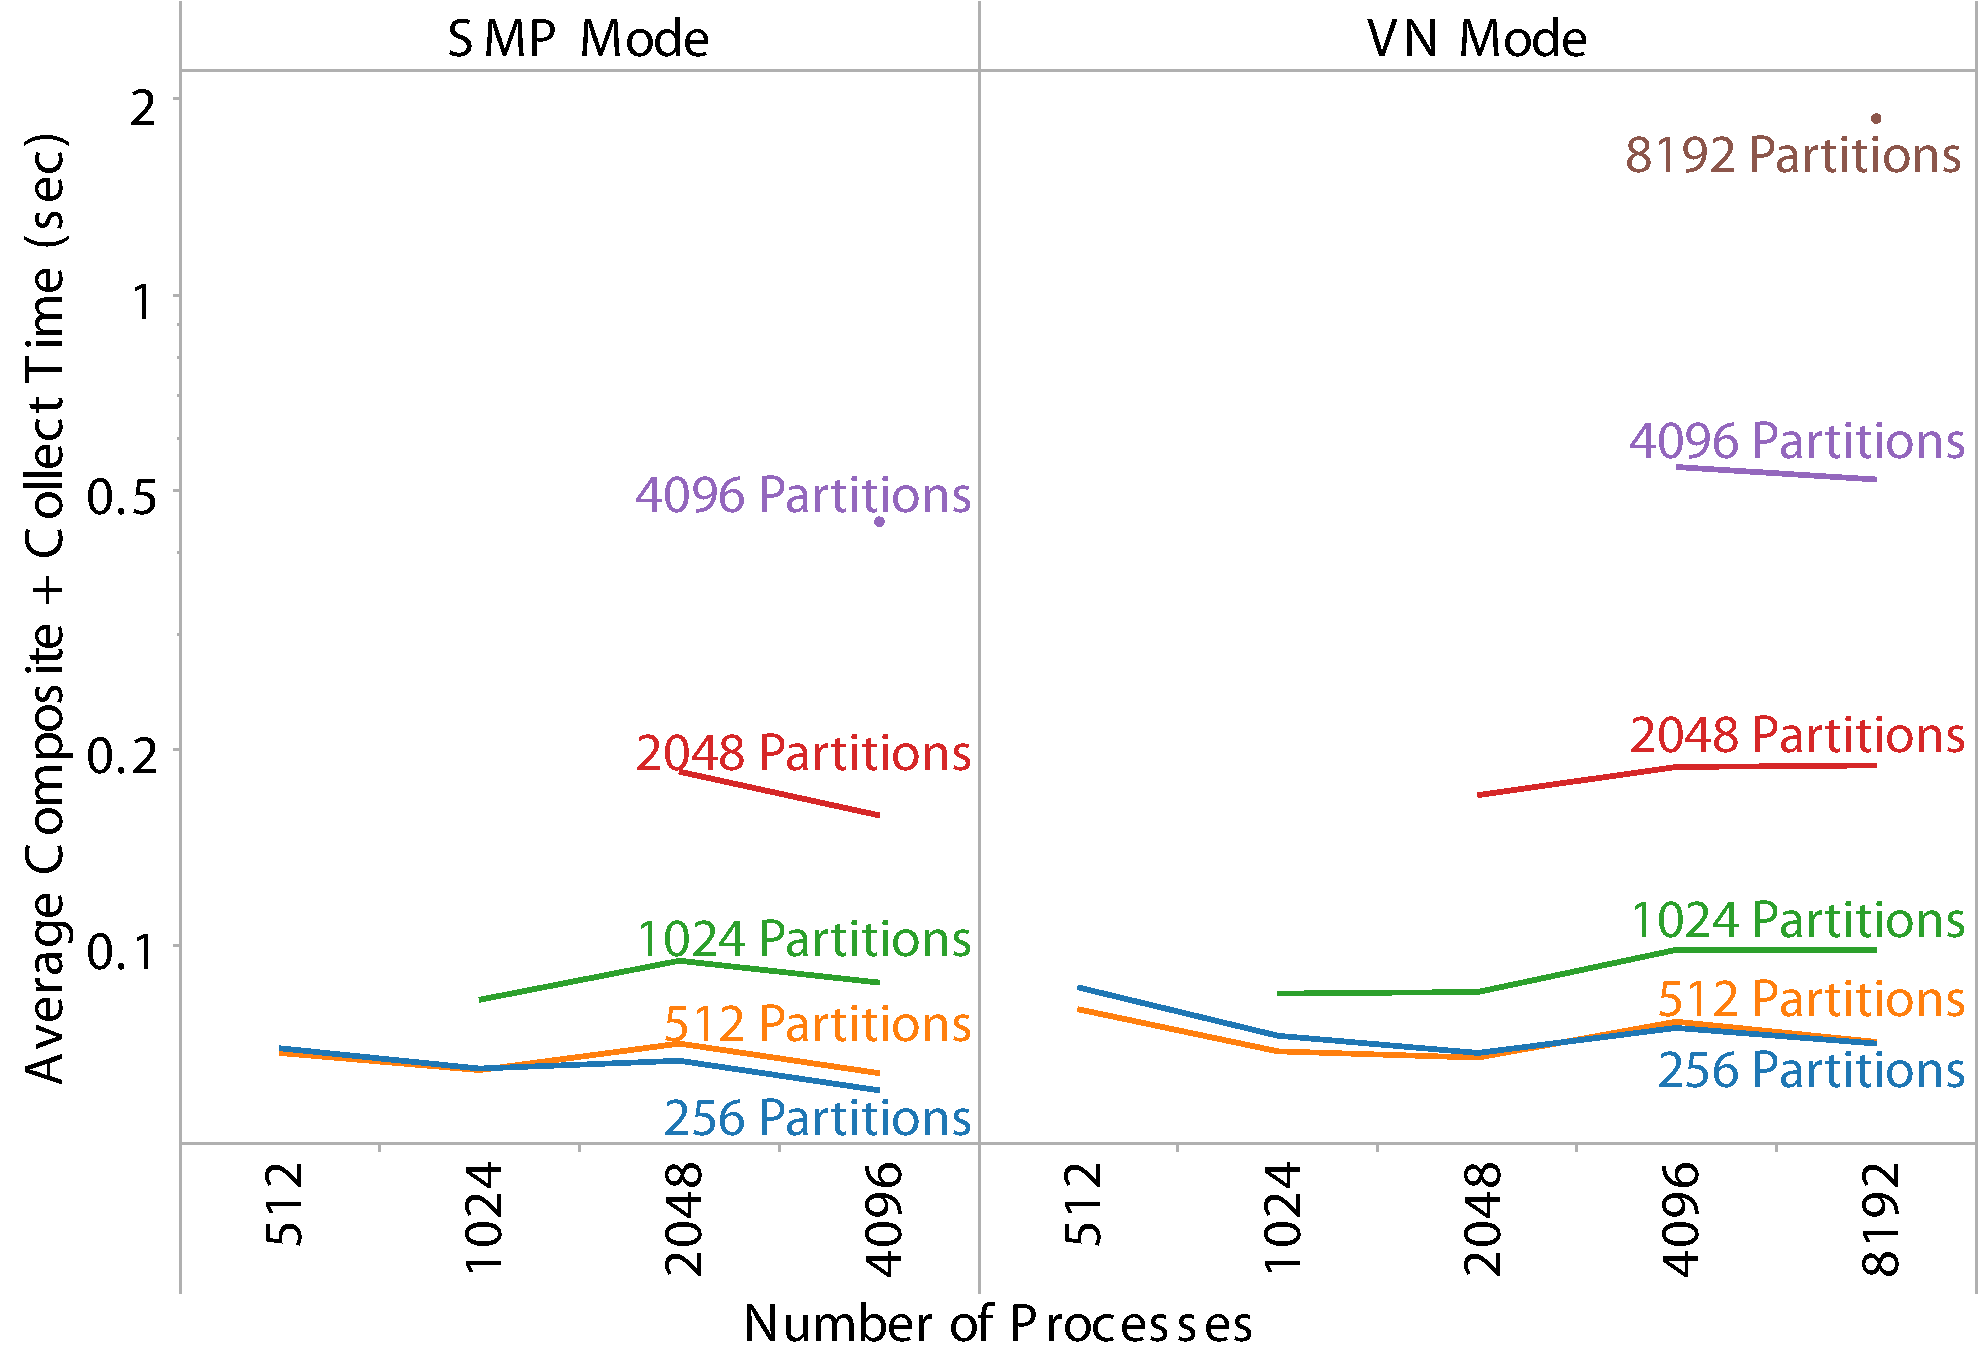
\includegraphics[width=\linewidth]{images/PartitionCollectIntrepidReduced}
  \caption{Compositing times on Intrepid when considering the time to
    collect image fragments into a single image and the total number of
    partitions is limited by collecting within rounds rather than
    splitting.  All times are given for binary swap.}
  \label{fig:PartitionCollectReduced}
\end{figure}

Figure~\ref{fig:PartitionCollectReduced} demonstrates the effects of
limiting the number of partitions on the binary swap algorithm (radix-k
with various values for $k$ is measured in the following section).  Due to
limits in processor allocation, we have not tested SMP mode with 8192
nodes, but other measurements suggest that the results will be comparable
to VN mode with 8192 cores.

Our best composite + collect measurements in
Figure~\ref{fig:PartitionCollectFull} occur at 512 partitions, so we
limited the maximum number of partitions to 256 and up.  Limiting the
number of partitions to collect clearly benefits the overall time for
larger process counts.  Our optimal number of partitions is in the 256--512
range.

\section{Scaling Study}
\label{sec:Scaling}

\begin{figure}[htbp]
  \centering
  \subfloat[Transparent Geometry]{
    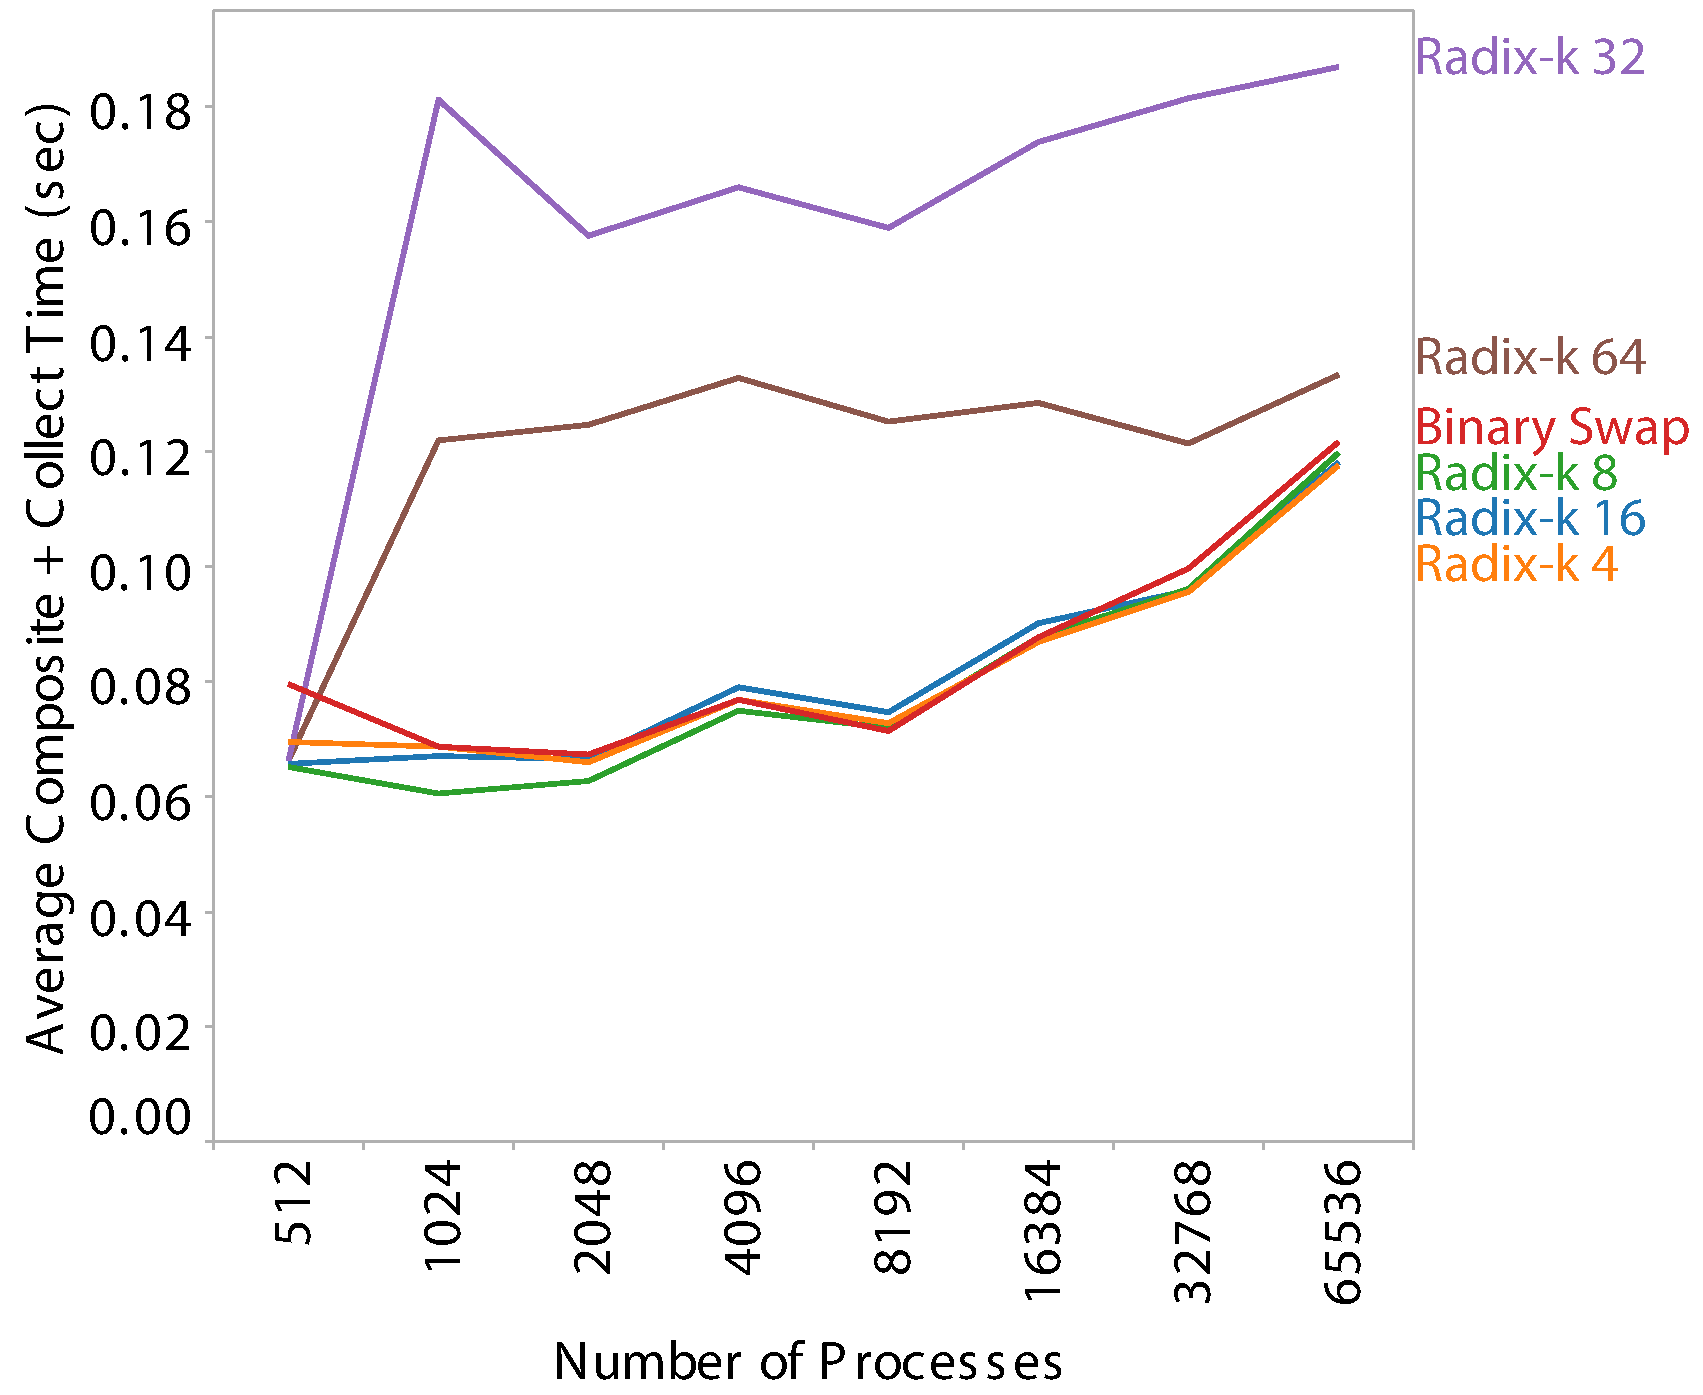
\includegraphics[width=.47\linewidth]{images/ScalingTransparent}
    \label{fig:Scaling:Transparent}
  }
  \hfill
  \subfloat[Opaque Geometry]{
    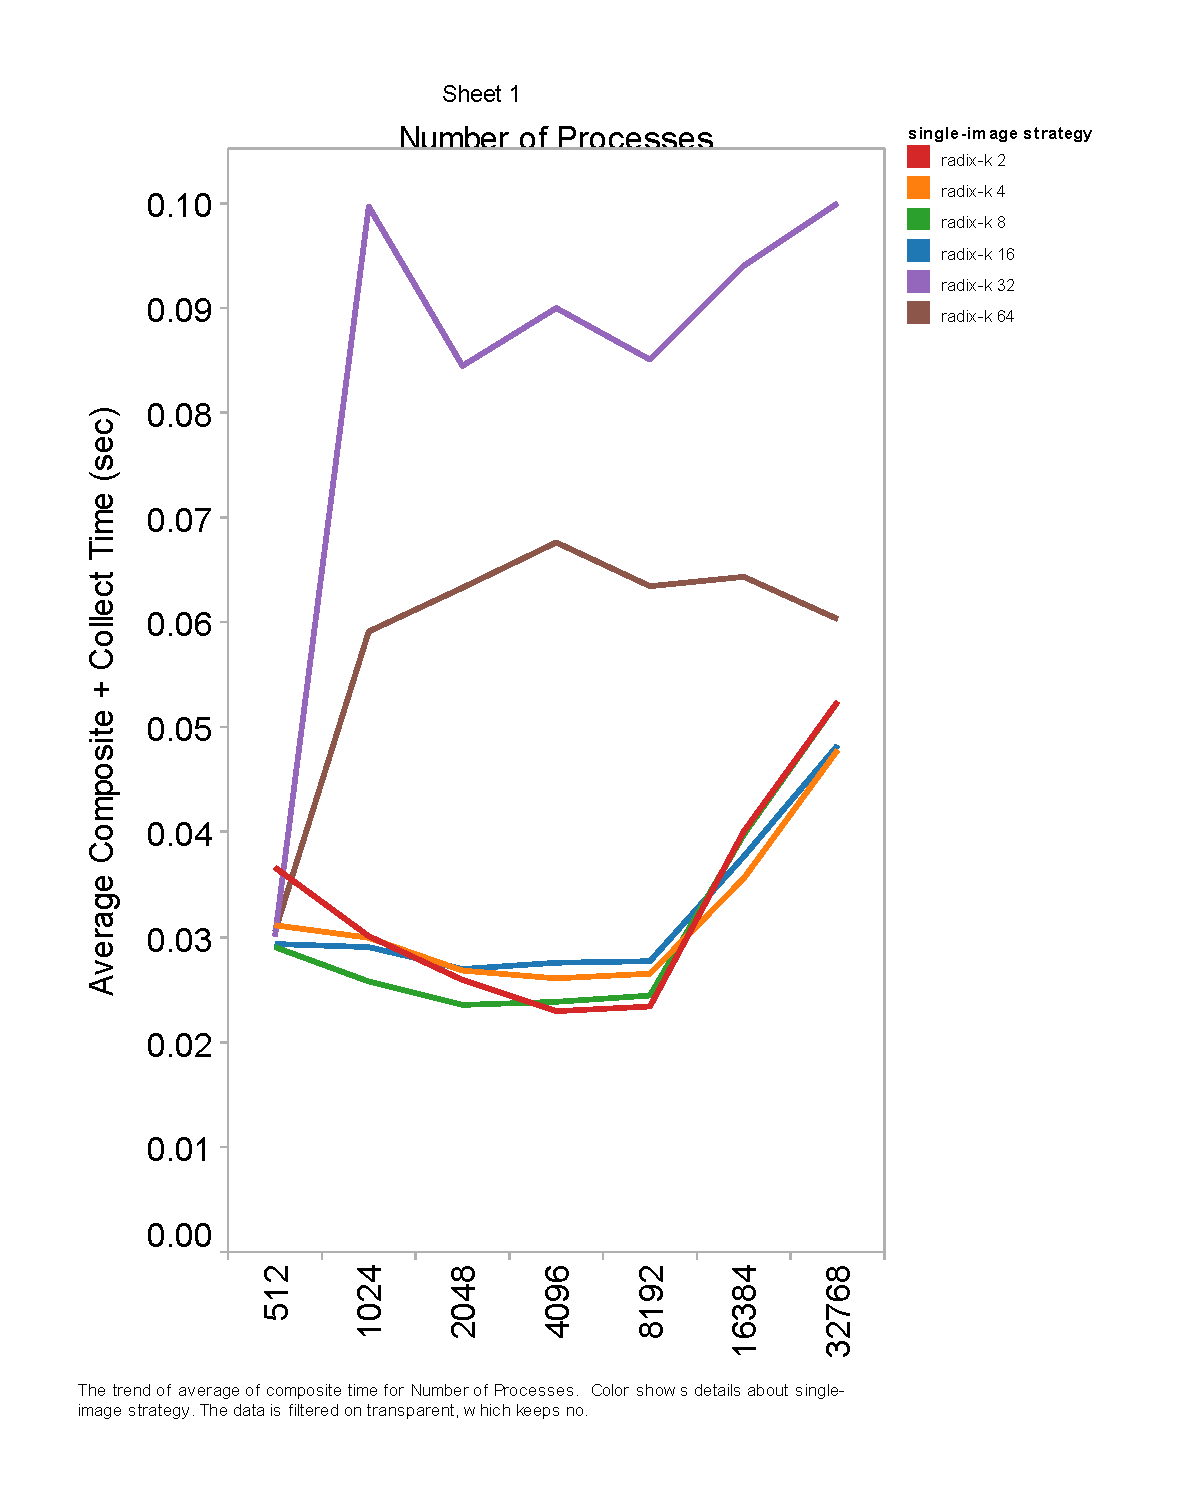
\includegraphics[width=.47\linewidth]{images/ScalingOpaque}
    \label{fig:Scaling:Opaque}
  }
  \caption{Performance of binary swap and several versions of radix-k on
    Intrepid up to 65,536 cores.  Transparent rendering uses 4 floats (16
    bytes) per pixel, and opaque rendering uses 4 bytes + 1 float (8 bytes)
    per pixel.}
  \label{fig:Scaling}
\end{figure}

For our final experiment, we observe the rendering system with all the
improvements discussed in this paper (except telescoping because we only
considered powers of two) scaled up to massive process counts.
Figure~\ref{fig:Scaling} summarizes the results.  Keep in mind that these
timings include collecting image partitions into a single image, a
necessary but expensive operation that is often overlooked.  All runs come
from Intrepid scheduled in VN mode.  For all runs we set the maximum number
of partitions to 512 although the actual number of partitions is smaller
with values of $k$ that do not factor 512 evenly.

For most runs, radix-k with $k=32$ and $k=64$ are significantly slower than
the others.  This is not an effect of the radix-k algorithm itself but
rather the maximum number of partitions that we used.  For example, two
rounds of radix-k with $k=32$ create $32 \times 32 = 1024$ partitions,
which is above our threshold.  Thus, the partition threshold is actually
throttled back to 32, which results in slower compositing that is not
compensated by faster collecting.

\begin{figure}[htbp]
  \centering
  \subfloat[Transparent Geometry]{
    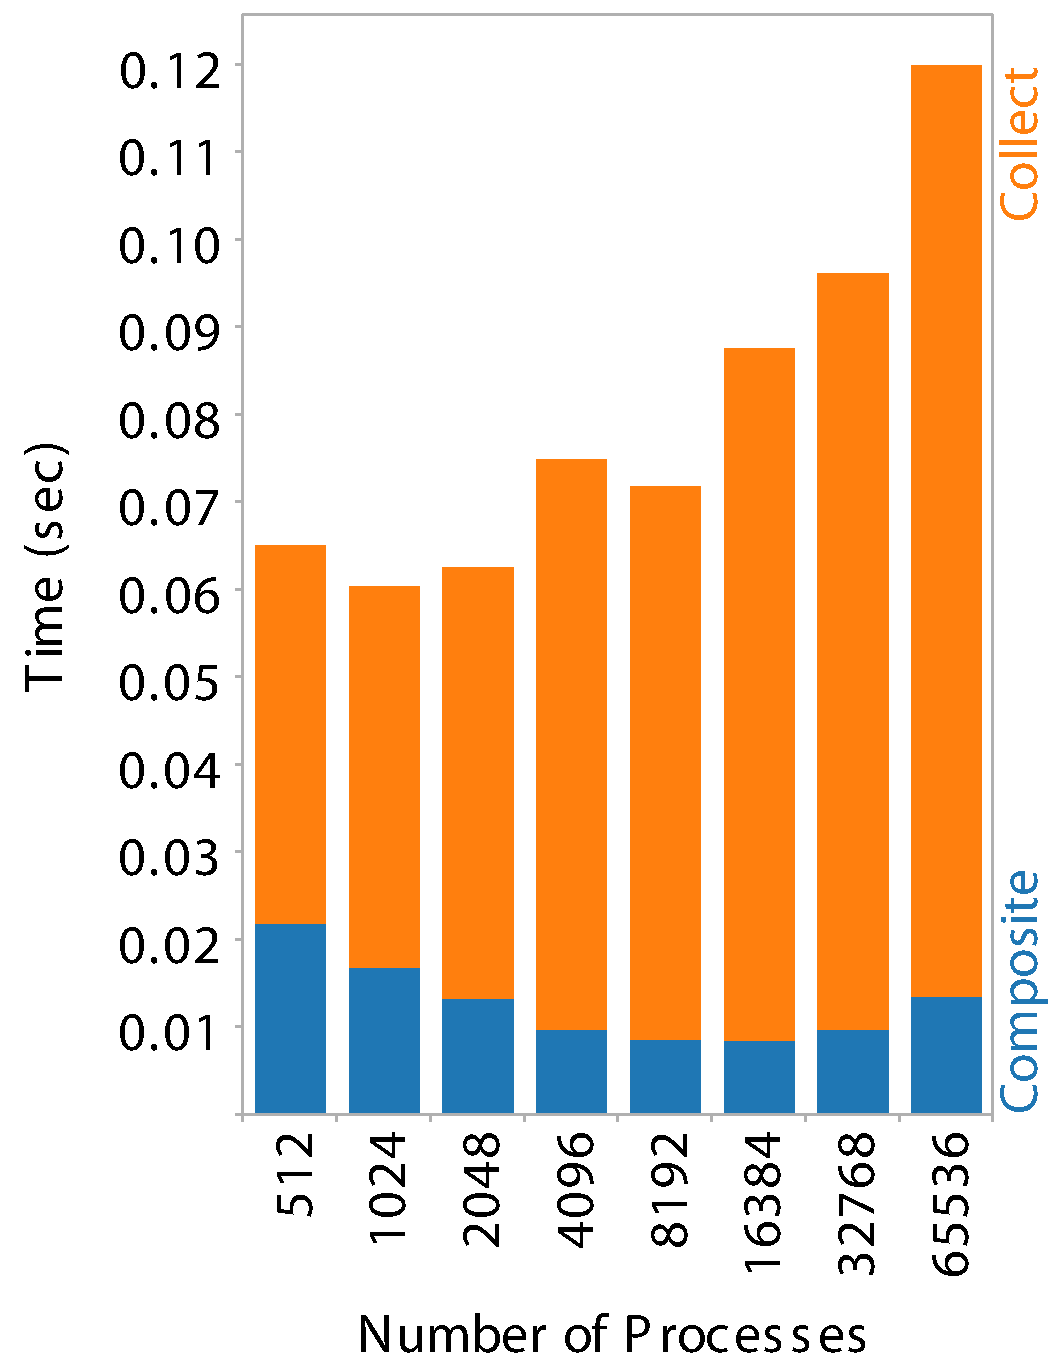
\includegraphics[width=.47\linewidth]{images/ScalingCollectTransparent}
    \label{fig:ScalingCollect:Transparent}
  }
  \hfill
  \subfloat[Opaque Geometry]{
    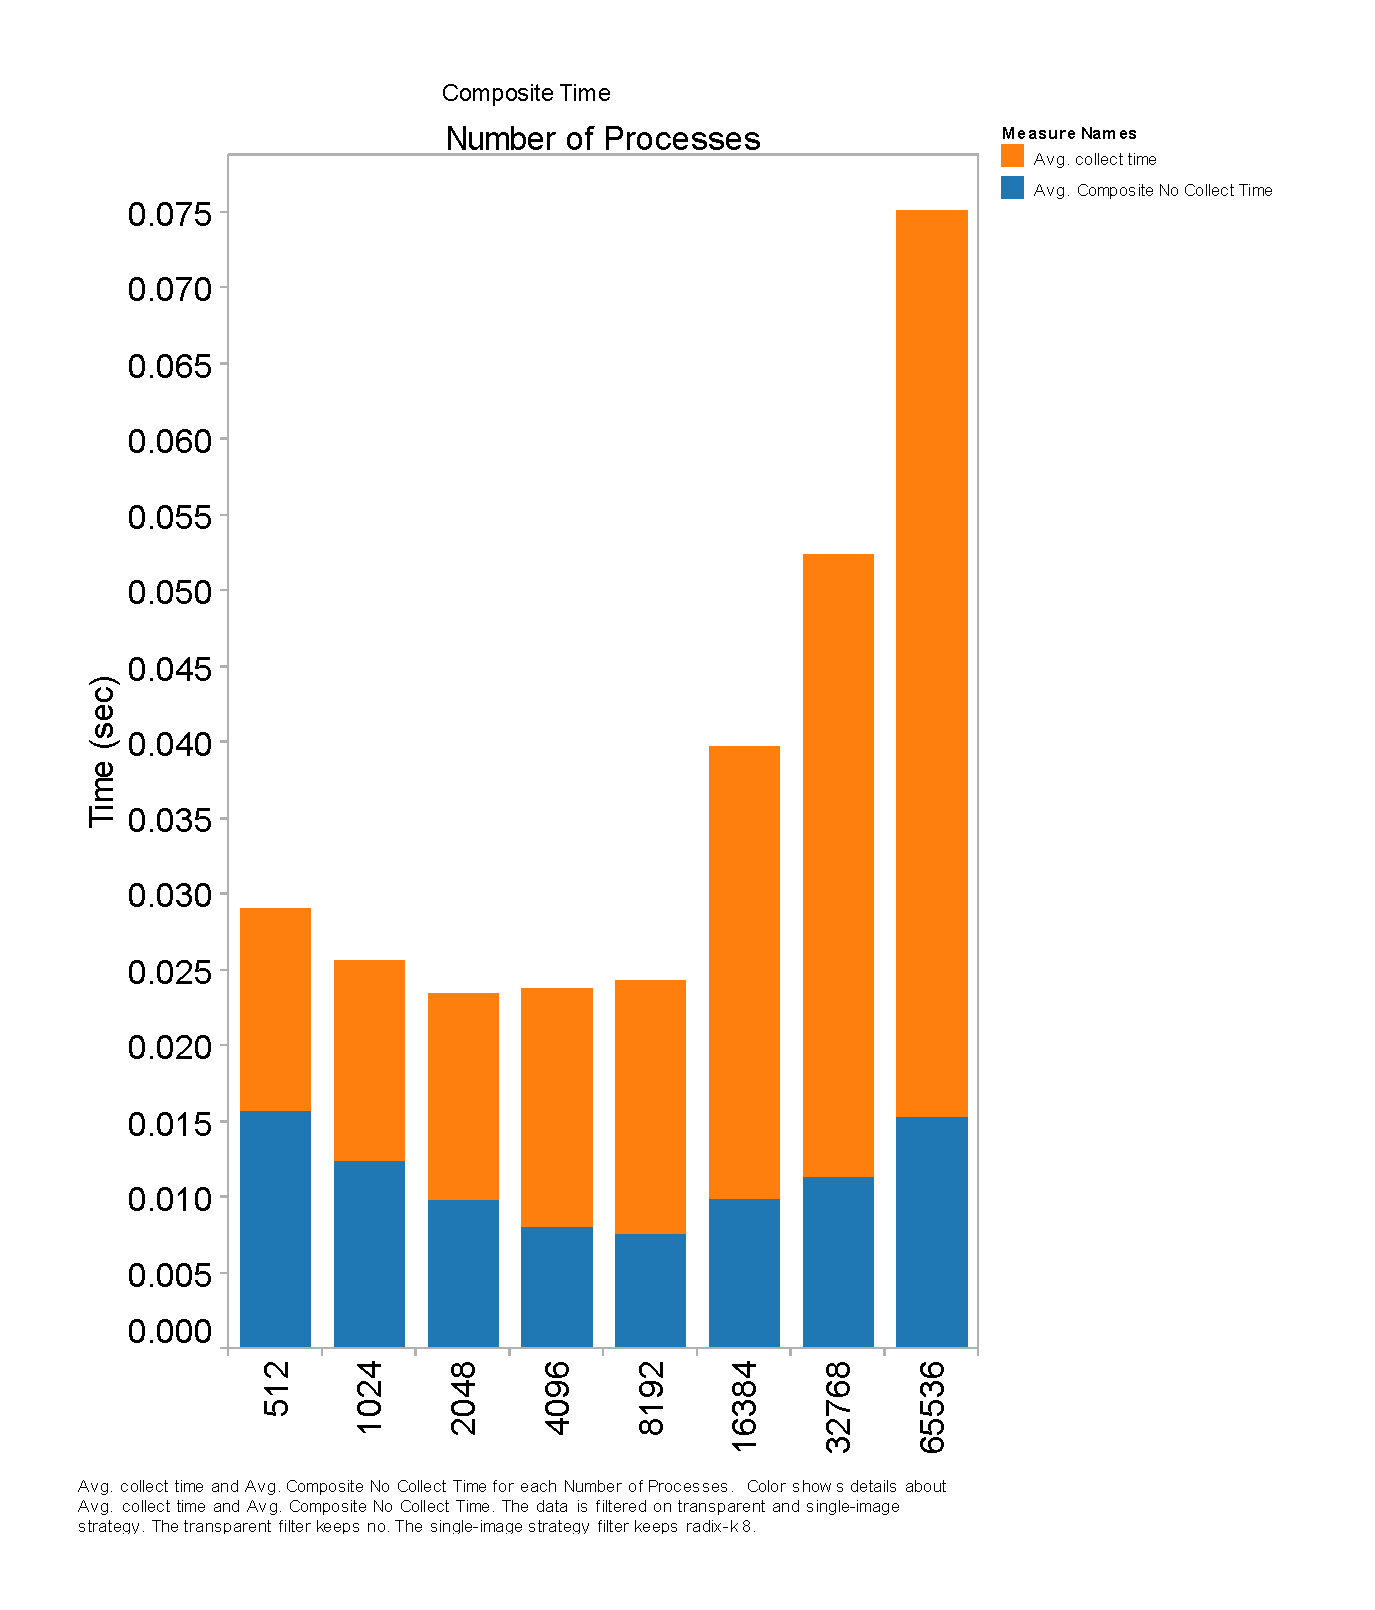
\includegraphics[width=.47\linewidth]{images/ScalingCollectOpaque}
    \label{fig:ScalingCollect:Opaque}
  }
  \caption{Performance of radix-k with $k=8$ on Intrepid up to 65,536
    cores.  Total time is divided into compositing and collection.}
  \label{fig:ScalingCollect}
\end{figure}

Our results show an increase in overall time for the largest process
counts.  This increase is primarily caused by an increase in collection
times despite our limits on the total number of partitions as is
demonstrated in Figure~\ref{fig:ScalingCollect}.  Nevertheless, we are able
to completely composite and collect an image on 65,536 cores in less than
0.12 seconds for transparent images (using floating point colors) and in
less than 0.075 seconds for opaque images (using 8-bit fixed point colors
and floating point depths).

\section{Conclusions}
\label{sec:Conclusions}

In this paper we describe several optimizations to image compositing for
sort-last parallel rendering.  We also demonstrate our completed system on
some of the largest process counts to date.  Our findings show that image
compositing continues to be a viable parallel rendering option on the
largest computers today.  These data also suggest a path for future
research.

The design of new fundamental compositing algorithms in addition to binary
swap, radix-k, and others is probably unnecessary.  In our observations,
the performance difference between binary swap and the various factorings
of radix-k are small compared to the other optimizations of the system such
as sparse pixel encoding, load balancing, and image collection.  In fact,
we find image collection to be the largest overhead currently in our
rendering system.  Addressing image collection is one of the most promising
avenues of future research.

Another fruitful area of research is better methods to take advantage of
multi-core processors.  Although it is reasonable to ignore the shared
memory between the four cores on Intrepid, future computers will have many
more cores per node.  Some introductory work has analyzed the behavior of
image compositing in shared-memory
architectures\lcite{Howison2010,Nouanesengsy2011,Reinhard2000,Peterka2008},
but further refinement is required to take advantage of the hybrid
distributed memory plus shared memory architecture of large systems and to
evolve the compositing as architectures and rendering algorithms change.

\section{Acknowledgments}

Funding for this work was provided by the SciDAC Institute for Ultrascale
Visualization and by the Advanced Simulation and Computing Program of
the National Nuclear Security Administration.
%
Sandia National Laboratories is a multi-program laboratory operated by
Sandia Corporation, a wholly owned subsidiary of Lockheed Martin
Corporation, for the U.S. Department of Energy's National Nuclear Security
Administration.
%
This research used resources of the Argonne Leadership Computing Facility
at Argonne National Laboratory, which is supported by the Office of Science
of the U.S. Department of Energy under contract DE-AC02-06CH11357.

\bibliographystyle{abbrv}
%\bibliographystyle{plain}
\bibliography{SLSmackdown}

\end{document}
